\documentclass[UKenglish]{ifimaster}
\usepackage[utf8]{inputenc}
\usepackage[T1]{fontenc,url}
\urlstyle{sf}
\usepackage{babel,textcomp,csquotes,duomasterforside,varioref,graphicx}
\usepackage[backend=biber,style=numeric-comp]{biblatex}
%\usepackage{color}   %May be necessary if you want to color links
\usepackage[hidelinks]{hyperref}
\usepackage{hyperref}
\usepackage{listings}
\usepackage{graphicx}
\usepackage{etoolbox}
\usepackage[newfloat]{minted}
\usepackage{caption}
\usepackage{multicol}
\usepackage{csvsimple}
\usepackage{pgfplots}
\usepackage[toc,page]{appendix}

\newlength\figureheight
\newlength\figurewidth
\pgfplotsset{compat=1.13} 

\hbadness=99999
\hfuzz=9999pt

\hypersetup{
   colorlinks=false, %set true if you want colored links
   linktoc=all,     %set to all if you want both sections and subsections linked
   %linkcolor=black,  %choose some color if you want links to stand out
}

\newenvironment{code}{\captionsetup{type=listing}}{}
\SetupFloatingEnvironment{listing}{name=Code}
\newcommand{\problemStatement}{One-Dimensional Convolutional Neural Networks on Motor Activity Measurements in Detection of Depression}

\title{\problemStatement}
\subtitle{
% Subtitle %
}

\author{Marie Ihle Frogner}
 
\bibliography{bibliography}

\begin{document}
\duoforside[dept={Department of Informatics},
program={Programming and Networks},
long]

\frontmatter{}
\chapter*{Abstract}
Teaching machines to learn patterns in data is very common these days, and it has a broad spectrum of applications everywhere. Sensors like smart-watches are getting more functionality each year, and more and more people buy them. Passing data from the watches, for example, activity or heart rate to machine learning algorithms, can generate significant results within many fields. Mental health is an example of a field where computer-generated predictions can be helpful to gain knowledge about patients. For example, machine learning can help predict that someone has a specific type of mental disorder.

In this thesis, we present applied machine learning to detect depression. The dataset (collected for another study about behavioral patterns in schizophrenia vs. major depression) contains motor activity measurements for each minute in the measured period for each participant. Three machine learning models are trained to fit time-sliced segments of these measurements. The first model classifies participants into  condition group (depressed) and control group (non-depressed). We trained another model to classify the depression level of participants (\emph{normal}, \emph{mild} or \emph{moderate}). Finally, we trained a model that predicts MADRS scores. We evaluate the performance of classification models using leave one participant out validation as a technique, in which we achieved an average F1-score of 0.70 for detecting control/condition group and 0.30 for detecting the depression levels. The MADRS score prediction resulted in a mean squared error of approximately 4.0. 

These performance scores are promising, but not good enough to be used in the real world. However, not much more work is needed for the first model if we apply it to a dataset with more participants.

\chapter*{Acknowledgements}
I would like to thank Pål Halvorsen and Michael Riegler for being my supervisors. Their feedback and tips have been essential for the success of my thesis.

Thanks to the developers of Grammarly. Their software has kept my writing at a decent level.

I would also like to thank my family and friends for motivating me and always believing in me. It has been difficult at times to stay focused on a large project like this.

My inner circle at IFI deserves a special thanks. We have been pushing each other through everything since day one, and we have now finished five years of education together.

\tableofcontents{} 
\listoffigures{}
\listoftables{}

\mainmatter{}
\part{Introduction}

\chapter{Introduction}
\label{chapter:introduction}
\section{Motivation}

The concept of Artificial Intelligence (AI) was introduced more than 80 years ago by among others Alan Turing \cite{turing1938}. We have come a long way when it comes to the type of technology, and AI is a heavily discussed topic today. Artificial \textit{General} Intelligence (AGI) is the concept of creating independent AI that can \textit{think} on its own, which many are either looking forward to or afraid of (probably because of movies like the Terminator), and we may not be that far away in terms of years from being able to build it \cite{peter_morgan_2019}. 

Machine learning (ML) is a sub-genre of AI where we \textit{train} computers to detect patterns in data quickly. One type of ML, deep learning, enables computers to beat humans in many games and predict outcomes of different events. 

Research on the usage of AI in the medical field is particularly interesting, as the results can be life-changing \cite{topol2019}. Instead of getting diagnosed only by a single doctor, an AI can influence their decisions. The difference between independent doctors worldwide would not matter as much, and with high accuracy, doctors could instantly know a lot about the patient. 

\emph{Three hundred and fifty million} people globally are fighting the burden of depression \cite{burden_of_depression}, which in a lot of the cases does not end well for them. ML has the potential here to help with diagnoses, help in the process of prescribing the optimal medicine to patients and predict whether a person is likely to attempt suicide \cite{topol2019}. 

There is no limit to the usefulness of ML in the medical field, and it can undoubtedly help in the field of mental health too. Consider bipolar disorder; a syndrome where a person experiences extreme mood swings. Say bipolar patients had a device that measured their heart rate among other things 24 hours a day could feed the data into a deep neural network that gave the user's bipolar state as output. That would be useful for both the patients and doctors/nurses. Using ML in this field of study could help many people get through their depression or mania, and potentially get rid of the condition altogether.

In summary, diagnosing bipolar patients is a challenge, errors are made, and it potentially takes a lot of time. However, much information can be extracted from simple sensor data measurements over a span of time, and in this respect, ML has great potential. 

We use ML to do experiments on recorded motor activity data from participants using a smartwatch. The included participants are divided into a condition group (participants with a mental condition) and a control group (participants without depression). With this data, we aim to detect which group participants are in, and also their severity of depression. The primary motivation for these experiments comes from earlier work done by Garcia-Ceja, E. et al. (\cite{GarciaCeja2018_classification_bipolar}), where they used ML to detect depression on the same participants. However, our usage of ML is different, and whether our performance is any better is a topic of discussion.

\section{Thesis Overview}
Based on the diagnosis challenges and the potential of ML on datasets collected from bipolar patients, we aim to find whether one specific type of ML, convolutional neural networks (CNN), together with motor activity measurements as input data, is a valid approach to detecting depression. We divide our goal into three objectives which we implement ML models to satisfy. We provide a walkthrough of the whole process, from data preprocessing to predictions and classifications from the trained ML models which we use to determine, for each objective, the final detected outcome of tested participants.

\begin{itemize}
    \item \textbf{The first objective} is to build a CNN model to detect depression. It should be able to detect (classify) whether a participant (where the motor activity measurements are unseen by the model while training) belongs to the control group or the condition group. We view this objective as the most relevant because it is the only objective that is comparable to earlier research.
    \item \textbf{The second objective} is to build a CNN model to detect \textit{levels} of depression. We divide the levels of depression into the following groups based on the Montgomery-Åsberg Depression Rating Scale (MADRS): no depression, mild, moderate and severe depression. The CNN should be able to classify the depression level of an arbitrary participant.
    \item \textbf{Our third and last objective} is building CNN model that predicts the MADRS score of participants. The main difference between the second and this goal is the architecture of the model. Instead of a classification model (multiple possible outcomes), we create a prediction model (one possible outcome, which can be any number). We evaluate this neural network by calculating the \textit{mean squared error (MSE)} of the predicted labels vs. the correct labels.
\end{itemize}

However, before getting started building CNN models, we experimented with linear regression. This type of machine learning can show whether variables are related to the target variable. In our experiment, we trained a linear regression model on several variables within the dataset to predict whether participants were in the control group or condition group (essentially the same as objective 1, only with linear regression). We achieved perfect performance with the models trained on the MADRS value of participants, which was an expected result.

We built a system that addresses the objectives defined above. This system uses \textit{real} data from depressed patients and non-depressed participants in order to see whether one can detect depression with ML.

We evaluate the performance of classification models (objective 1 and 2) using a \textit{leave one participant out} technique combined with majority voting. In the first objective, we achieved an F1-score of 0.70, which is promising but it still has room for improvement. The second objective resulted in an F1-score of 0.30, which is significantly worse than the first. However, as described in chapter \ref{chapter:training}, this model detects non-depressed participant correctly at a high performance. For the third objective, we achieved an MSE of approximately 4.0, which is also promising. 

The reported performance indicates that motor activity measurements can give useful information about mental health issues. However, the results are only at best promising. Applying our ML models in the real world needs to happen together with experts, especially for the second and third objectives. 

\newpage

\section{Thesis outline}
In \textbf{chapter \ref{chapter:background}}, we provide background information about mental health and ML. In mental health, we describe the topics of bipolar disorder and how the Montgomery-Åsberg Depression Rating Scale can tell patients how depressed they are. Then we introduce important topics within ML, and how easy it is to get started writing models in Keras, a ML framework for Python. Related work is the last section in chapter 2, where we mention several papers related to the topics of mental health and ML. \\

\noindent \textbf{Chapter \ref{chapter:planning}} is where we describe the objectives that we want to achieve in the thesis. We present the dataset we use to achieve those objectives, and also how we structure and preprocess the data so that it can be used to train models. Performance metrics that we use later in order to evaluate a trained model is another topic we define in the chapter.\\

\noindent \textbf{Chapter \ref{chapter:models}} contains a description of the neural network model for each objective in addition to a linear regression model. We describe all layers in the models and include the source code used to create them in the ML framework Keras. \\

\noindent In \textbf{chapter \ref{chapter:training}}, we walk through how we trained the models in order to reach our objectives, then evaluated them with metrics described in chapter 3. \\

\noindent \textbf{Chapter \ref{chapter:discussion}} is where we discuss whether convolutional neural networks can be used to classify and predict mental health issues. We also suggest real-world applications of our work, focusing on the pros and cons of creating and trusting an AI for mental health diagnoses. \\

\noindent \textbf{Chapter \ref{chapter:conclusion}} contains our conclusion and a summary of the chapters, and we give directions for future research.

\chapter{Background}
\label{chapter:background}

The fields of studies for this thesis are both mental health and ML, and this chapter contains background information and previous research within both of them. We start with mental health, where we describe mental issues, depression, and bipolar disorder. Then we dive into the topic of ML, where we provide a technical introduction.

\section{Mental health}
Mental health problems are not known very well by the public. Jorm et al. performed research \cite{jorm1997mental} where they displayed vignettes of one patient suffering from major depression and one from schizophrenia to the people of the Australian public. Of the participants, only 39\% correctly guessed depression, and 27\% correctly guessed schizophrenia. Another study has shown that schizophrenia is often confused with multiple personalities \cite{angermeyer1999social}. Such poor public knowledge about mental health problems can be problematic, as people may have a condition without knowing anything about it. When this is the case, professional help use more time to establish their diagnosis. 

\subsection{Depression Rating: MADRS}
Montgomery-Åsberg Depression Rating Scale, or MADRS for short, is a rating system for telling how depressed a patient is. Stuart A. Montgomery and Marie Åsberg designed it in 1979, and it is more sensitive to changes than the Hamilton Rating Scale for Depression (HRS) for patients that go through antidepressant medication. The process for calculating a MADRS rating contains ten statements about the patient's behavior, where the topics are: apparent sadness, reported sadness, inner tension, reduced sleep, reduced appetite, concentration difficulties, lassitude, inability to feel, pessimistic thoughts, suicidal thoughts \cite{madrs_paper}.


The person doing the rating answers each question with a number between 0 and 6, where the higher the number, the more relevant the statement is for the patient. The numbers added together gives us the total MADRS score, which we split into four categories: normal/not depressed: 0-6, mild depression: 7-19, moderate depression: 20-34 and severe depression: 34-60 \cite{sunnybrook_stroke_study}. 

\subsection{Bipolar Disorder}

Bipolar disorder is the syndrome with extreme mood swings, referred to as \emph{mania} and \emph{depression} \cite{bipolar_disorder}. One day the person can feel amazing, and everything is fine, 
but the next day they feel like they do not belong anywhere in this universe. In general, one should be concerned about mood swings. 
It is, however, the extreme cases where the mind turns 180 degrees from day to day that is the main symptom of bipolar disorder. 
There is not a specific type of people that get this; they can be of any age and any gender, but most people that suffer from it find out 
(by having an experience or episode) around age 25 \cite{bipolar_statistics}. 

When talking about bipolar disorder, we often separate between the states \emph{normal}, \emph{mania} and \emph{depression}. 
The last two are the states we usually talk about since a normal state is not that interesting. These two states are very different, 
but they have some similarities, for example sleeping problems. When a bipolar person is in a manic state, they may feel so excited and powerful that they do things that they would never have intended doing, like spending much money on items they do 
not need \cite{bipolar_disorder}.

A bipolar patient is in a depressive state when they are in a bad mood swing. They can stop doing everything they usually like to do, 
and lie down in bed all day with no motivation to do anything useful. They may feel useless and that they do not belong here, 
or being guilty of something they may or may not have done. In some cases, depression may even end up with suicidality, 
where the person either spends much time thinking of death, or attempt suicide.

The frequency of these symptoms can vary. One year they can have these mood swings every day for several weeks at the time, and the next they get them less frequent, 
like once every month. We also separate between bipolar disorder type I and II, with the main difference being that the manic episodes are way 
more aggressive in type I \cite{bipolar_types}. Statistics say that bipolarity is genetically inheritable, with 23\% chance of getting a child with bipolar 
disorder if one parent is bipolar, and 66\% if both parents are \cite{bipolar_statistics}. 

\section{Machine learning}
ML is the field of computer science where we throw data into an algorithm and expect it to give answers to whatever the goal is, 
with as little work as possible. The process of performing ML was not as simple in the early days of the technology, 
but nowadays it is a lot easier with all the different frameworks and tools available.

ML is a tremendous and almost magical technology, but knowing how one should use it can be difficult without the experience. 
The amount of data needed to make an algorithm learn something makes it difficult to get started, and to be efficient when training the model on a large dataset, 
decent hardware is required. One can get away with using a CPU if they want to test ML on a small dataset, but if the goal is to build something useful, 
too much time is saved using a GPU. 

The reason why GPUs are so much better than CPUs on this specific task is that the design choices of a CPU are for flexibility and general computing workloads. 
The GPU, on the other hand, is designed to do simple arithmetic instructions over and over again (easy to parallelize). These design choices make GPUs a lot more 
efficient for ML, and especially for deep neural networks \cite{cpu_vs_gpu_ml}. Alternatively, if investing in a GPU is not the preferred choice, 
there are many cloud services available to us today where we can pay a small sum in order to use a system that is a better fit for the task.

Now how do we make a machine learn? Well, there are many different approaches to this, which we will discuss in the next sections, but let us say we want to 
use a neural network for achieving some goal. Then our next step should be to choose a framework. We can, of course, do everything from scratch, but why 
reinvent the wheel when there are so many good frameworks and tools already out there? 

Python is a programming language perfect for ML in our opinion. The language looks a lot like pseudo-code, and this is perfect because we do not 
want to spend time on syntax rules in another language. A popular framework called \textbf{TensorFlow} is available to use in Python, and developers from Google have built it. 

TensorFlow allows the programmer to build models quickly, and also execute the training and testing. TensorFlow can be used directly, but using \textbf{Keras} as an abstraction layer above it is a popular choice, which we did when implementing the neural networks for our objectives. On their documentation website \cite{keras_docs}, they describe their framework as \blockquote{A high-level neural networks API, written in Python and capable of running on top of TensorFlow, CNTK or Teano}.

Following their \textit{30 seconds to Keras} guide \cite{keras_docs}, you can create a \textit{sequential} model with \textit{dense}
layers, configure its learning process (compile), then fit, train, evaluate and predict with just a few lines of code \ref{code:keras-guide}.

\begin{figure}
  
\begin{code}
  \begin{minted}[linenos]{python}
      from keras.models import Sequential
      from keras.layers import Dense
  
      model = Sequential()
  
      model.add(Dense(units=64, activation='relu', input_dim=100))
      model.add(Dense(units=10, activation='softmax'))
  
      model.compile(loss='categorical_crossentropy',
                optimizer='sgd',
                metrics=['accuracy'])
      
      model.fit(x_train, y_train, epochs=5, batch_size=32)
      loss_and_metrics = model.evaluate(x_test, y_test, batch_size=128)
      classes = model.predict(x_test, batch_size=128)
  \end{minted}

  \caption{Simple introduction to Keras, where we create a Sequential model with two Dense layers, compile it with with the loss function Categorical Crossentropy and the optimizer SGD \cite{keras_docs}.}
  \label{code:keras-guide}
\end{code}
\end{figure}

One thing that Keras does not make any easier is structuring the dataset so that the model can fit it. There is a high chance that we have to write some 
code ourselves to do this. Numpy is a package for Python built for math operations where everything happens optimally (Python by itself adds overhead to everything). 
All Python based ML algorithms assume that the input data is Numpy arrays, so experience with Numpy can be advantageous when structuring the dataset.

\section{Machine learning strategies}
Picking the right ML model can be quite tricky, especially for an inexperienced programmer. There are a couple of different \textit{strategies} one can choose 
from when deciding on an ML model. These are called \textit{supervised and unsupervised learning}, and we need to think about how the dataset is structured, 
and what we want to achieve to find out which one to use. The following sections will be a description of the strategies, to make the decision easier.

\subsection{Supervised learning}
Supervised learning is the ML strategy where we provide both input and correct output data to the algorithm \cite{supervised_learning}. 
We may use supervised learning if the goal is to train a model to classify letters in the alphabet, or something else where we have a dataset with both input 
and output data (for the alphabet, images of letters are input data, and the actual letters are the output data). If we train this alphabet detection model, 
we will be able to input an image (not seen before by the algorithm) of a letter, and the model will classify it to the letter it most likely correct. 
This kind of supervised learning is called \textit{Classification} and is the problem of assigning new observations to the class they most likely belong, 
based on a classification model built from labeled training data \cite{supervised_learning}.

Another kind of supervised learning is called \textit{Regression} and is all about predicting (or estimating) a value. A classic example of regression 
learning is predicting income, using \textit{features} like home, location, job title, the field of study,  years of education and years of experience. 
We call these features \textit{categorical} (first three) and \textit{numerical} (last two) \cite{supervised_learning}. 

\subsection{Unsupervised learning}
Another strategy is unsupervised learning. We want to use this if we have a dataset without the same meaning as in a dataset for supervised learning. 
The items may not have a fixed answer, like the letters in the alphabet are. It is useful when we have unlabeled data and want to for example group data 
together in what we call a \textit{cluster}. Unsupervised learning may not be as common as supervised learning, but it can be quite 
beneficial in some cases; for example when grouping addresses together in neighborhoods if we have an unsorted list of addresses as the dataset. Patterns are given to the algorithm, but no \textit{answers} are provided \cite{unsupervised_learning}. 

\subsection{Semi-supervised learning}
We may not always want to use one of the strategies above. Looking at the dataset, maybe we want something in between like a combination of labeled and unlabeled data. Semi-supervised learning comes in handy when this is the case. For example, if we have many data samples to label in our dataset, it can be too much work. We will not go deep into details about how this works, but it is essential to mention it because of its usefulness. The goal of semi-supervised learning is to understand how combining labeled, and unlabeled data may change the learning behavior, and design algorithms that take advantage of such a combination \cite{semisupervised_learning}.

\section{Machine learning approaches}
When we know whether we want to use supervised learning, unsupervised learning or something in between, we need to select an approach. We use the term approach because we use these regardless of the strategy, as most approaches work in both supervised and unsupervised learning. There are a lot of different approaches available, and we will describe some of them.

\subsection{Decision tree learning}
\begin{table}[h]
    \centering
    \begin{tabular}{| l | l | l | l | l | l |}
    \hline
    \textbf{Day} & \textbf{Temperature} & \textbf{Outlook}   & \textbf{Humidity}  & \textbf{Wind}     & \textbf{Run} \\ \hline
            1    & 15 C                 & Sun                & Low                & Strong            & Yes \\
            2    & 6 C                  & Rain               & High               & Weak              & No  \\
            3    & 15 C                 & Rain               & Medium             & Strong            & Yes \\
            4    & 6 C                  & Overcast           & High               & Medium            & Yes \\
            5    & 15 C                 & Sun                & Low                & Weak              & No  \\
            6    & 12 C                 & Overcast           & Medium             & Weak              & No  \\
            7    & 12 C                 & Sun                & Medium             & Medium            & Yes \\
    \hline
    \end{tabular}
    \caption{Example training data set: days a person went out for a run}
    \label{table:days_running}
\end{table}

In computer science, trees are data structures commonly used to describe something that \textit{branches out} based on different input. For example, 
a tree can be a representation of how the frequency of letters in the alphabet are distributed in a text file so that the text file can be compressed optimally. 
We will not go into details about how this works, but our point is that tree-structures are very common in most fields of computer science. 

In ML, we can apply the tree-structures as \textit{decision tree learning}. Decision trees are trees that classify instances by sorting them based on feature values, and each \textit{node} represents a feature. Each branch represent a value that the node can assume \cite{supervised_learning}.
In this approach, we set up all the different outcomes (with the training data set) of a specific question in a tree. Let us say we want to predict whether or not a person will run outside on a specific day. 
Then it makes sense that the training set contains weather information. The different data in the training set is called attributes, and correctly picking 
these is essential for the quality of the prediction.

Table \ref{table:days_running} contains data about whether a person went outside for a run or not for a week (just an example, not real data). 
Here the first 4 (excluding "Day") columns (Temperature, Outlook, Humidity, and Wind) is the "predictors" and the last column (Run) is the target. 
To use this table in decision tree learning, we need to view it as a tree, with one of the predictors as the root node and the targets as leaf nodes. 

How we choose the tree structure is critical to the performance of the ML, and we need to use a good tree building algorithm. 
The most common algorithm to use in this situation is the \textit{ID3} algorithm made by J. R. Quinlan. It is a top-down, greedy search through the space 
of possible branches with no backtracking \cite{decision_tree}. The way this happens is by calculating \textit{Entropy} and \textit{Information Gain}. 
The idea is to recursively choose the predictor that has the highest information gain and generate a tree structure. With an optimal tree, 
we can create decision rules by merely following the tree with new data.

\subsubsection{Random Forest}
One known problem with decision tree models is that they often include much \textit{variance}. Variance in an algorithm means that it is sensitive to small 
changes in the training set. One method to reduce the variance is to use Random Forest. 

Random forests are a combination of tree predictors such that each tree depends on the values of a
random vector sampled independently and with the same distribution for all trees in the forest \cite{random_forest}. 
It is a supervised ML strategy and can be useful for both classification and regression learning.

For example, if we want to get movie recommendations using ML, using one decision tree will most likely be insufficient. 
Just think what happens when we ask a friend for movies to watch. What that friend recommends is purely based on movies we like ourselves and what the friend likes. 
We might be lucky and find our next favorite movie, but most likely, asking multiple people for recommendations is going to yield better results. 
The same goes for ML, and decision trees will most likely give a better answer if we combine them in a Random Forest.

\subsection{Deep Neural Networks}

\begin{figure}[!ht]
    \begin{center}
        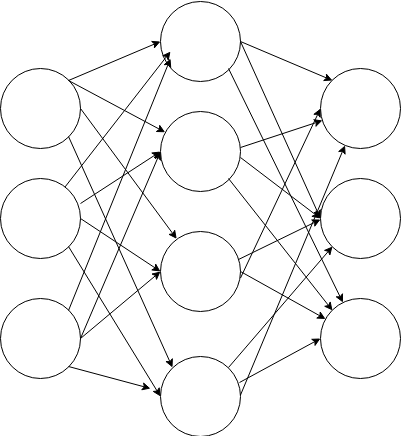
\includegraphics[height=10cm]{neural_net.png}
        \caption{Neural network visualization. The inputs on the left side are passed into the neurons in the hidden layer in the middle, which passes the values to the output layer.}
        \label{figure:neural_net}
    \end{center}
\end{figure}

The general idea of ML with neural networks is to make the computer think like a human, inspired by the way biological neural networks in the human brain process information \cite{deep_learning}. There are a lot of different neural network architectures, but all of them share the same underlying layer-based architecture, where data get passed between layers where computation happens. The first layer is the input layer, which passes the data to the next layer, which is the hidden layers. The number of hidden layers is entirely up to the model and the programmer, and this is where the intermediate processing/computation is done before the data get passed to the output layer where we perform an activation function to define the output \cite{deep_learning}.

Figure \ref{figure:neural_net} is a visual representation of a neural network with the input layer on the left, one hidden layer in the middle and the output layer on the right-hand side. For each layer, we have fully connected nodes, which means that each node has a connection to all nodes in the next layer.

If we have multiple hidden layers in a neural network, we call it a \textit{deep} neural network (DNN). DNNs can be useful for anything, and only the programmer's creativity sets the limit. Two common ways to use DNNs are \textit{Recurrent Neural Networks (RNNs)} and \textit{Convolutional Neural Networks (CNNs)}. These two have their use cases, which we will describe further.

\subsubsection{Recurrent Neural Network (RNN)}
RNNs are useful for predicting something based on a sequence of data, like for example predicting words in a sentence, which can be especially useful for typing on the phone. Also making predictions based on historical data, speech and language, are tasks an RNN can do effectively \cite{deep_learning}.

One downside to RNNs used on large sequences of data is that the prediction will most likely be off if a word written at the beginning of a long text is a dependency for a prediction four chapters later, for example, the home location of the main character. The workaround for this is something called \textit{Long Short-Term Memory Recurrent Neural Network (LSTM RNN)}, and is the idea of having additional logic to avoid the prediction model forgetting essential facts \cite{deep_learning}.

\subsubsection{Convolutional Neural Network (CNN)}
A CNN can be used for identifying patterns in data, which then is the underlying calculations for either prediction or classification. They are designed to process data in different array shapes \cite{deep_learning}. A common use case for CNNs is image recognition. In image recognition, we train our models to be good at identifying objects in images, for example, the difference between cats and dogs. Then we can input a completely different image to the model, and it will output whether the image is of a cat or a dog. 

This type of CNN is two-dimensional because an input image is a two-dimensional array of pixels, so the network also needs to have two dimensions in the convolutional layers. Another way of constructing a CNN is one-dimensionally, which can be useful for \textit{one-dimensional} data, for example, sensor data from gyroscopes or accelerometers \cite{deep_learning}.

\begin{quote}
\textit{A 1D CNN is very effective when you expect to derive interesting features from shorter (fixed-length) segments of the overall dataset and where the location of the feature within the segment is not of high relevance. This applies well to the analysis of time sequences of sensor data (such as data from gyroscopes or accelerometers).} \cite{1d_cnn}
\end{quote}

For this reason, we decided on implementing one-dimensional CNNs to achieve the objectives of our goal. Also, the results are important, as no researchers have applied CNNs on motor activity measurements in the field of mental health yet to our knowledge. 

\section{Related work}
In this section, we mention several research papers that are related to these two topics Mental Health Monitoring Systems (MHMS) and CNNs.

\subsection{Mental Health Monitoring Systems}
In the field of MHMS, research has already been done by many. In this subsection, we describe some earlier research about depression/bipolar disorder, where they also applied machine learning to their study. 

E. Garcia-Ceja et al. surveyed some of the recent research works in machine learning for MHMS \cite{GarciaCeja2018_survey}. They gave the different works labels: study type (association/detection/forecasting), study duration (short-term or long term), and sensor types (wearable/external/software or social media). 

Association studies were those who help understand the relationships between variables, and the methods include linear regression, correlation analysis, t-tests and analysis of variance. Detection studies have a goal to detect/recognize the mental state, often using methods like classification models. Forecast studies aim to predict events about patients, for example, epileptic seizures. The wearable sensor types include smart-watches and smartphones, external sensors could, for example, be cameras or microphones installed in an institution where the participants were patients. Some studies, where the sensor type was software or social media used services like Instagram to collect their data \cite{GarciaCeja2018_survey}. 

To find relevant work for this thesis, we had a look into some of the studies included, which studied depression and bipolar disorder. One study by O'Brien, J.T. et al. \cite{obrien_depression} was an association study about depression, where the participants wore accelerometers on their wrists. Twenty-nine adults with depression and 30 healthy adults participated, and the goal was to study the possibility that physical activity has an impact on depression (referred to as Late Life Depressions (LLD) in the paper). They found that the physical activity of participants with LLDs was significantly lower, which is highly relevant for this thesis because our dataset contains physical activity data. 

Grünerbl, A. et al. had a detection type study about bipolar disorder \cite{grunerbl_smartphone_bipolar}. The participants consisted of ten bipolar patients in Austria between 18 and 65 years old. In this study, the recorded data was phone calls and microphone data and achieved average recognition accuracy of 76\% and precision and recall of over 97\% of bipolar state detection. They also used the accelerometer and GPS as input data and achieved recognition accuracy of 70\% (accelerometer) and 80\% (GPS).

In a study by Maxhuni, A. et al. \cite{maxhuni2016}, they used the same participants as the previous example. The difference was that in addition to using accelerometer and microphone data, they introduced questionnaires to the participants. For the results, they applied different machine learning algorithms, and their best average accuracy was 85.57\%.

Faurholt-Jepsen, M. et al. had an association type study about bipolar disorder \cite{faurholt_smartphone_bipolar}. The participants were 29 bipolar patients, and actions on their smartphones like daily usage, the number of incoming calls, the number of text messages sent and received. They found correlations between the mental state of the patients and the recorded information. 

Andrew G. et al. applied machine learning to photos posted on Instagram \cite{instagram_depression}. They had 166 participants, who posted a total of 43,950 photos. By extracting statistical features using colors analysis, metadata and face detection, they achieved models that outperformed the average practitioner's success rate when diagnosing depression (70\% of all depressed cases identified). Research on social media usage in the field of mental health is interesting because, for many, those are the platforms that they use to express their feelings. 

Mowery, D. et al. did another study based on social media \cite{twitter_depression}, but instead of Instagram, they used Twitter. For a tweet, they classified whether or not it contained evidence of depression, and there was evidence of depression, they classified one of three symptoms (mood, disturbed sleep or loss of energy). The features they extracted from each tweet included \textbf{syntax} (usage of first/third person pronouns), \textbf{emoticons} usage (happy/sad), and \textbf{sentiment} (whether the text was subjective/objective and positive/negative). They achieved the best performance when classifying that a tweet had no evidence of depression, and their other models performed significantly worse. 

The authors of the paper mentioned first surveying different machine learning research in MHMS, Garcia-Ceja, E. et al., also released a paper on motor activity based classification of depression in unipolar/bipolar patients \cite{GarciaCeja2018_classification_bipolar}. They applied machine learning for classifying depressed/non-depressed participants using Random Forest and a DNN. The dataset is the same as we used here in this thesis (described in detail in the next chapter), and they achieved an F1-score of 0.73 with Random Forest and 0.7 with the DNN. Since one of our objectives is to do the same classification as in this paper, it was worth mentioning.

The main difference between earlier research within MHMS and our work is that we aim to apply a CNNs to achieve our goal. CNN is a type of machine learning that is more sophisticated than the ones used in the mentioned research papers. We know that motor activity measurements can be related to mental health issues (from Garcia-Ceja, E. et al. \cite{GarciaCeja2018_classification_bipolar}). However, the best methods for extracting this type of knowledge is not known. With our experiments, we want to find if CNNs can do this job effectively.

\subsection{Convolutional Neural Networks}

In most of the papers previously mentioned, the complexity of the machine learning models has not been the area of focus, but rather comparing different algorithms like decision trees and Naïve Bayes. A study by Kiranyaz, S. et al. used a 1-D CNN on real-time patient-specific ECG (electrocardiogram) classification \cite{ecg_1d_conv}. While this paper is not in the field of mental health, we found exploring how others have created CNNs helpful for us when building our models. Kiranyaz, S. et al. achieved superior classification performance comparing it to most of the state-of-the-art methods, and concluded with the fact that after training a CNN dedicated to a patient, it can be solely responsible for classifying their ECG records.

Human activity recognition (HAR) is another field of study where machine learning has shown its value. Ronao, C. A. et al. presented a deep convolutional network \cite{ronao_har_conv} for classifying human activity (walking, sitting, standing and laying) based on a 1-D time-series of measurements from smartphone sensors. The accuracy they achieved on their test set (95.75\%) outperformed the previous state-of-the-art models. 

The usage of convolutional networks is, of course, not limited to the medical field. Ince, T. et al. published a paper on real-time motor fault detection using a 1-D CNN \cite{motor_fault_conv}. They used raw signal data as input to the model, and a model that only has to be trained once for each motor they achieved an accuracy of detecting motor faults above 97\%.

All of the mentioned CNNs have high performance, which is a promising indication for our results. The type of data that we apply our CNN to is very similar to the HAR study by Ronao, C. A. et al. \cite{ronao_har_conv}, but we use it in the detection of mental health issues instead of human activity. 

\section{Summary}
In this chapter, we described background information and related work for our goal. We mentioned different mental health problems, but we focused on depression. Within the topic of depression, we described a rating system called MADRS and then gave an introduction to bipolar disorder. Furthermore, we discussed ML: how one can get started using the Keras ML framework in Python, and different ML strategies and approaches. At the end of the chapter, we discussed related work within the topics of MHMS and CNNs. 

We learned about how MADRS provides a systematic way of telling how depressed patients are, which is essential to know as we use the MADRS score of participants in objective two and three. Bipolar disorder was also necessary to gain knowledge about because some of the participants have the diagnosis. From the topic of ML, we are going to apply a supervised learning strategy, with a DNN approach, and more specifically a CNN type network to achieve our goal. 

Before we can train a CNN, we need to structure the input and output data. In the next chapter, we present a description of the dataset, then discuss our methods of how the system fulfills the objectives by preprocessing the input and output data, and evaluate performance after training has completed. 

\part{Methodology}
\chapter{Planning and Preparing Data}
\label{chapter:planning}
\begin{figure}[h]
  \begin{center}
      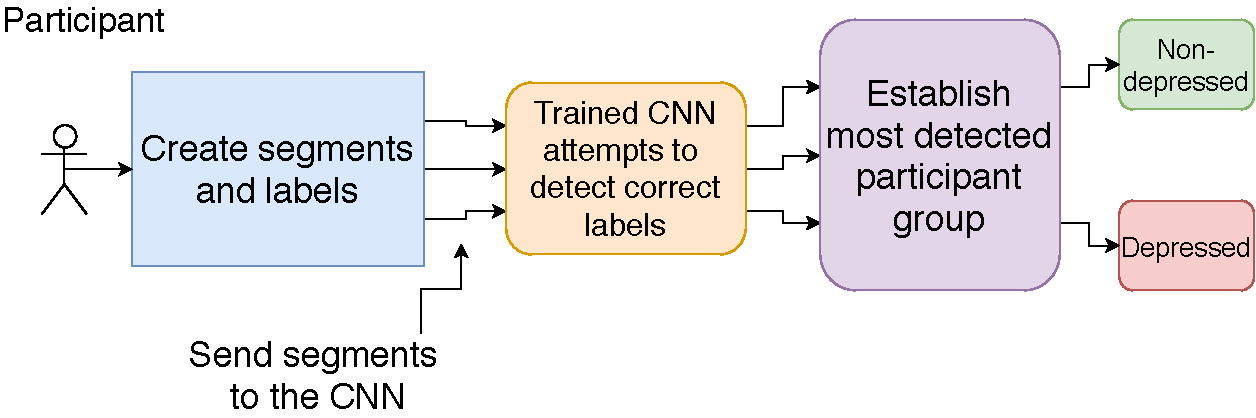
\includegraphics[height=4cm]{img/flow_detection.pdf}
      \caption{Diagram of how we detect whether a participant is depressed or not (first objective) after we have trained the CNN. }
      \label{figure:flow}
  \end{center}
\end{figure}

\noindent As described in chapter \ref{chapter:introduction}, our objectives in this thesis include creating three CNN models:

\begin{itemize}
  \item Detect whether a participant is depressed or not.
  \item Detect whether a participant has no depression, mild depression, moderate depression or severe depression.
  \item Predict a participant's MADRS score.
\end{itemize}

\noindent We also implemented a linear regression model that trained explicitly on the demographic data. The reason for this experiment, which does not include a CNN, was to see if we could learn from any column whether the participants are depressed or not. This experiment is further explained in chapter \ref{chapter:models}. 

For our CNNs, the input data is processed into time-sliced segments of motor activity measurements. Then we send the segments to the CNNs, which attempts to detect the correct value for each segment. During the training process, correct values have to be visible to the model for it to learn (because we use a supervised learning strategy). After training the models, they should be able to classify/predict the correct value depending on the objective. Because we split the measurements of a participant into segments, we needed to gather all of the detected value so that we could return one final detection. Majority voting is the method used for this, which means that we use the most popular detection (label with most \textit{votes}). How the system works from A to Z detecting whether a participant is depressed or not is visualized in figure \ref{figure:flow}.

We implemented one-dimensional CNNs that were able to take the segments of activity data as input. Also, we wanted the neural network models to be as similar as possible. With few changes in the layers (preferably only the last few layers), we could use a model on another objective. It was, however, only possible for the first two objectives, as they are both about classification and we only changed the number of units in the output layer. We changed more layers for the third objective. We describe of all neural network models in detail in chapter \ref{chapter:models}.

In this chapter, we describe the structure of the dataset, how we use the dataset to create activity segments, and how we can test and evaluate the performance of machine learning models.

\section{The dataset}

\begin{figure}[!ht]
  \centering
    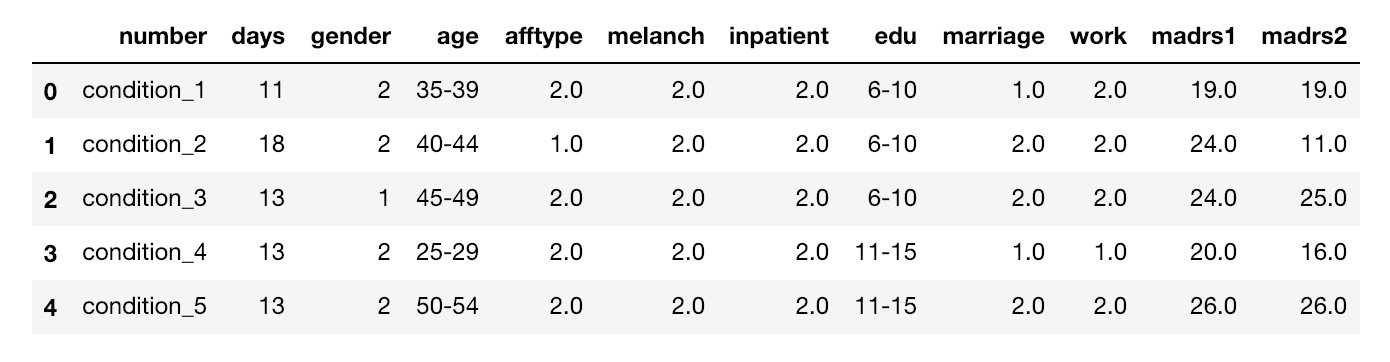
\includegraphics[height=3.5cm]{img/demographics.png}
    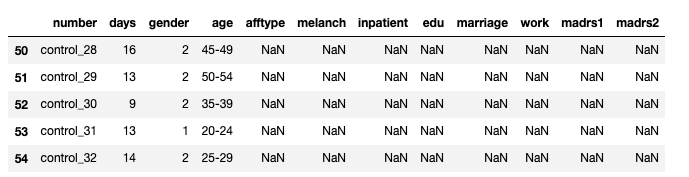
\includegraphics[height=3.5cm]{img/demographics_control.png}
    \caption{The 5 first and the 5 last rows in demographic dataset (scores.csv). The displayed participants are from the condition group (above) and control group (below).}
    \label{figure:demographics}
\end{figure}

\begin{figure}[!ht]
  \centering
  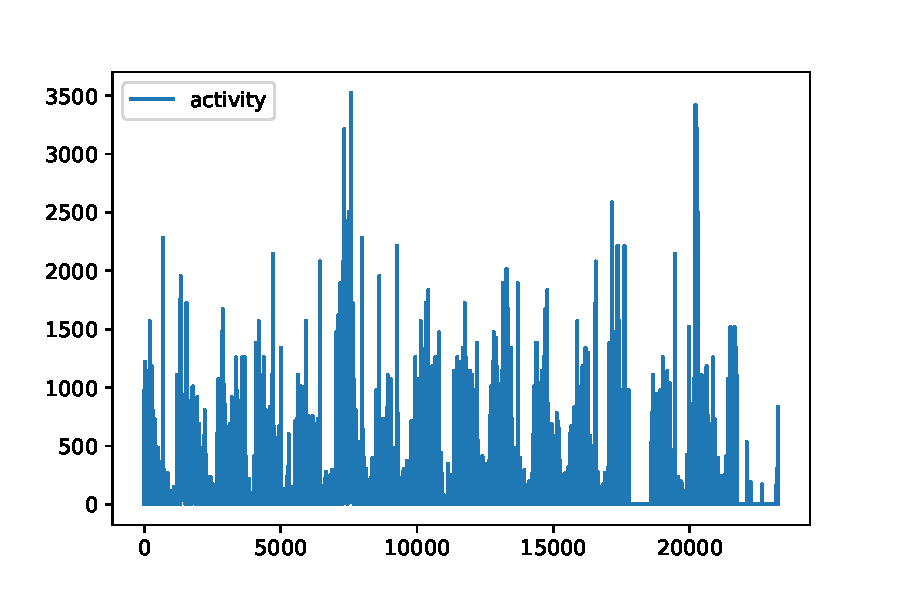
\includegraphics[height=6cm]{img/activity_condition_1.pdf}
  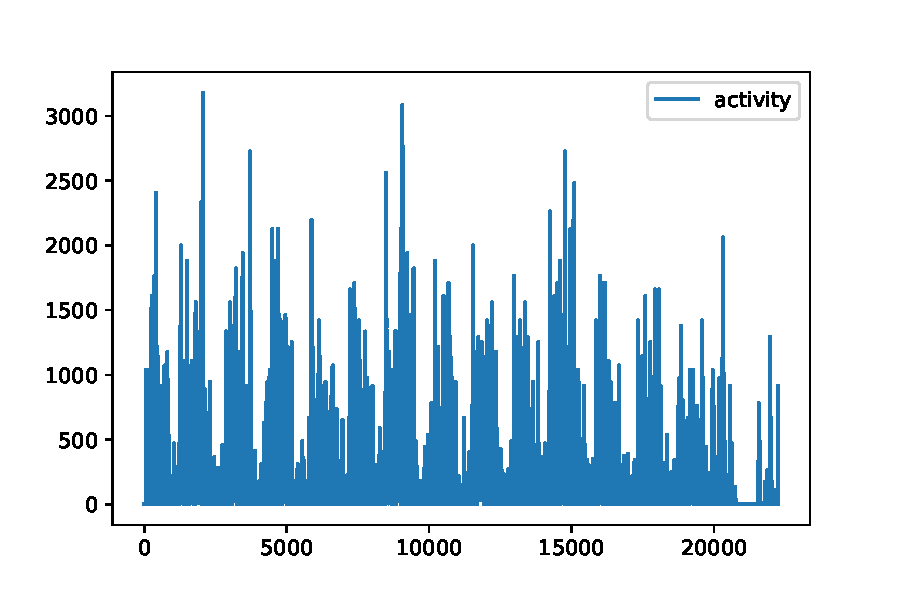
\includegraphics[height=6cm]{img/activity_control_1.pdf}
  \caption{Motor activity measurements for a participant in the condition group (above) and control group (below). The condition group participant is male between 35 and 39 years old, diagnosed with unipolar depression. The control group participant is female between 45 and 49 years old. The number on the X-axis corresponds to the minute throughout the measurement period, and the number on the Y-axis is the activity levels.}
  \label{figure:participant_activity}
\end{figure}

In this thesis, we used a dataset (called \textit{Depresjon} after the Norwegian word for depression) containing motor activity measurements from participants wearing an Actiwatch (model AW4 from Cambridge Neurotechnology Ltd, England). The dataset was collected originally for a study about behavioral patterns in schizophrenia vs. major depression \cite{Berle2010}. The participants we focus on are 23 bipolar/unipolar patients and 32 non-depressed contributors, removing the participants with schizophrenia. We will refer to the bipolar/unipolar group as the \textit{condition group}, and the non-depressed group as the \textit{control group}. Garcia-Ceja et al. also follows this convention in their work \cite{GarciaCeja2018_classification_bipolar}.

The dataset is in two parts. One part includes the demographics of each participant (see figure \ref{figure:demographics}), where the fields are:

\begin{itemize}
    \item \textbf{number}: a unique id for each participant
    \item \textbf{days}: number of days of data collection 
    \item \textbf{gender}: 1 = female and 2 = male
    \item \textbf{age}: age of the participant (grouped by four years)
    \item \textbf{afftype}: affliction type, where 1 is for bipolar type II, 2 equals unipolar depressive, and 3 for participants with bipolar type I
    \item \textbf{melanch}: 1 means a participant has melancholia, 2 means no melancholia
    \item \textbf{inpatient}: whether the patient is inpatient (1) or outpatient (2)
    \item \textbf{edu}: how many years of education the participant has completed (grouped by four years)
    \item \textbf{marriage}: married/cohabiting (1) or single (2)
    \item \textbf{work}: whether the participant is working/studying (1) or not (2)
    \item \textbf{madrs1}: MADRS score before activity measurement started
    \item \textbf{madrs2}: MADRS score after activity measurements ended
\end{itemize}

The second part of the dataset includes motor activity measurements about participants in the condition group and control group, as one file for each participant. These files are placed in two folders for the two groups respectively, and there is one file for each participant with filename as "GROUP\_X.csv" where X is their id and GROUP is either condition or control. Inside each file, we can find a list of motor activity measurements for every minute of the data collection period.

Looking at example participants from both groups (figure \ref{figure:participant_activity}), we can not immediately tell with our eyes that they are different. However, by feeding the data into a CNN, we aimed to find patterns that were specific to the two participant groups. 

\section{Data Preprocessing}
\label{section:data_preprocessing}

We wrote a function (see source code in appendix \ref{code:reading_dataset}), which was responsible for preparing the data before we sent it into the neural network. We started by defining a \textit{segment length} ($L$), which is how much data (minutes) we want inside each segment. We experiment with the value of $L$ in chapter \ref{chapter:training}. Next, we needed a value for how many indexes to step after each iteration, $S$. We kept this value at one hour, meaning $S=60$. Between the different objectives, this function will only be different in how it yields the \textit{labels}.

\begin{itemize}
  \item First we read the \textit{global} dataset, where we find each participant and whether they are in the control or condition group. As there is no \textit{afftype} value for non-depressed participants, we set this to 0. Other possible values are 1, 2 and 3. We do the same for the \textit{madrs2} column.
  \item Then we iterate over the participants:

  \begin{itemize}
    \item Build segments and labels arrays for current participant:
    \begin{itemize}
      \item Append a segment that is of length $L$ to the list of segments. 
      \item Append a value to labels depending on the objective (see the subsection about output data).
      \item Increase the index by $S$, then repeat until we have added all segments for the current participant.
    \end{itemize}
    \item Example element in segments and labels for a participant in the condition group: \\
    \textbf{segments[i] = [[0], [143], [0], [20], [166], [160], [306], [277]]}\\
    \textbf{labels[i] = [[1], [1], [1], [1], [1], [1], [1], [1]]}
  \end{itemize}
  
  \item Make the list of labels into a \textit{categorical} 2D matrix (see table \ref{table:categorical_labels}) with a \textbf{1} in only one of the columns, instead of a single-dimensional list. This is only needed in the first two objectives.
\end{itemize}

\begin{table}[h]
  \begin{center}
    \begin{tabular}{| l | l |}
      \hline
      \textbf{Control group} & \textbf{Condition group}  \\ \hline
      0                    &  1                \\ \hline
      1                    &  0                \\ \hline
      0                    &  1                \\ \hline
      1                    &  0                \\ \hline
      1                    &  0                \\ \hline
      0                    &  1                \\ \hline
      0                    &  1                \\ \hline
      1                    &  0                \\ \hline
    \end{tabular}
    \caption{Categorical Labels. A 0 and a 1 (first row) means that the participant is in the condition group.}
    \label{table:categorical_labels}
  \end{center}
\end{table}

The output data was an array with a value for each segment, corresponding to the objective and the participant. After creating it, we used a helper function from Keras called \textit{to\_categorical} to transform the array into a categorical matrix instead of a list of labels. Table \ref{table:categorical_labels} is an example of how a categorical matrix looks. The value we used to build this array was based on the objective:

\begin{itemize}
  \item For classifying control/condition group, this list was built to contain the values \textbf{0} or \textbf{1} for the labels \textbf{CONTROL} and \textbf{CONDITION}, which was chosen according to the group the participants were in. For example, \textbf{labels[i] = [0, 1]}, meaning that segment $i$ is labeled as \textbf{CONDITION} group. 
  
  \item To classify depression classes, we used MADRS scores divided into four classes by some cutoff-points:
  \begin{itemize}
    \item 0-6: normal
    \item 7-19: mild depression
    \item 20-34: moderate depression
    \item 34-60: severe depression
  \end{itemize}
  So instead of labelling the segments as \textbf{CONTROL} or \textbf{CONDITION}, we labeled them as \textbf{NORMAL}, \textbf{MILD} and \textbf{MODERATE} (we ignored severe depression as there are no participants with MADRS scores this high). An example element in this array after applying \textit{to\_categorical()} is \textbf{labels[i] = [0, 1, 0]}, which means that segment $i$ is labeled as \textbf{MILD} depression.
  \item For predicting MADRS scores, we built the array of the MADRS score of the participants. Example: \textbf{scores[i] = [18]}.
\end{itemize}

\section{Performance}

When finishing with a training session for a machine learning model, we need to use different metrics to be able to tell how the model performed based on some testing data. For prediction models, we only consider the value returned by the \textit{loss function}, but evaluation of classification models can be presented with several metrics. In this section we present loss functions and optimizers, and how we evaluate the performance of our models using classification metrics and different ways of splitting up into training and testing data.

\subsection{Loss functions and Optimizers}

After defining a machine learning model, we \textit{compile} it so that it was ready to be \textit{fit} to the dataset. Compiling a model requires a \textit{loss function} and an \textit{optimizer}. The loss function is the function that evaluates how well the model \textit{models} the given data \cite{loss_functions}, and the optimizer is the function that attempts to lower the output of the loss function. 

For the first two objectives in this thesis, we use the loss function \textit{categorical cross-entropy}, which calculates a probability over the number of classes supplied (number of classes equals the number of neurons in the output layer) \cite{cross_entropy}. In the third objective, we use a loss function called \textit{Mean Squared Error (MSE)}, which is measured as the average (mean) of squared difference between predictions and actual observations \cite{loss_functions}. The formula below is used to calculate the MSE, where $n$ is number of training samples, $i$ describes the current element in the samples, $y_i$ is true label for the current sample and $\hat{y}_i$ is the predicted label for the current sample.

\[ MSE = \frac{\sum_{i=1}^{n}(y_i-\hat{y}_i)^2}{n} \]

When choosing an optimizer, there are many different options available, but we chose an optimizer called \textit{Adam} for training all of our models. Adam is an algorithm for efficient stochastic gradient-based optimization \cite{adam}, and it is available as an optimizer function within the Keras framework \cite{keras_docs}. The reason for choosing Adam is, as described by Kingma, D. P. et al. \cite{adam}, efficient both considering memory usage and computationally. The hyper-parameters also require minimal tuning. Using a different optimizer can make the model fit the dataset at a different pace, which is something we experiment with in chapter \ref{chapter:training} (for the third objective). 

\subsection{Classification metrics}
In classification, accuracy is a metric that is commonly used. It makes sense to the human brain; telling a friend that has no experience in machine learning or data science that we have made our computer able to classify something with 98\% accuracy is something that they would understand. Other metrics include \textit{precision}, \textit{recall}, \textit{specificity} and \textit{F1 score} \cite{GarciaCeja2018_classification_bipolar}, which will be described below.

\subsubsection{Confusion matrix}

\begin{figure}[h]
  \begin{center}
    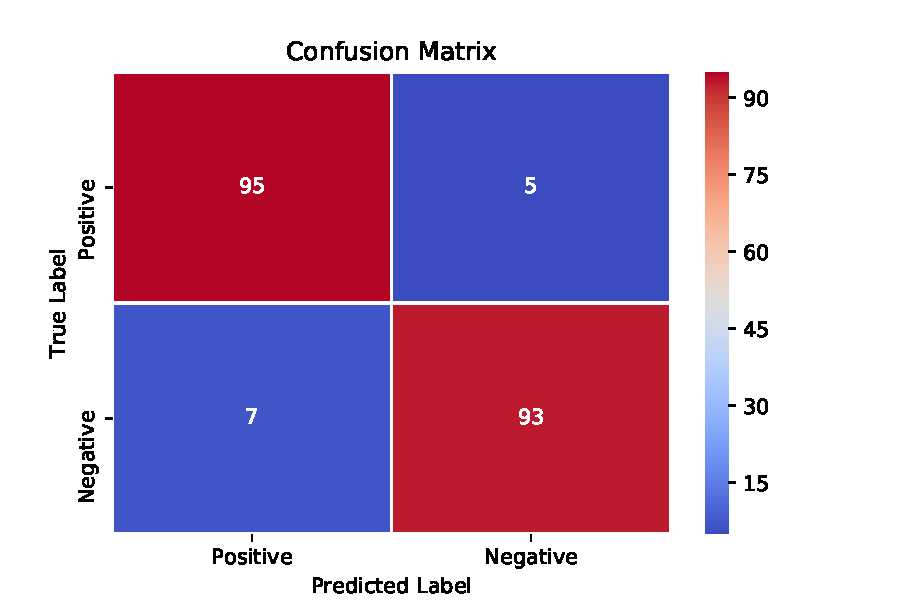
\includegraphics[height=8cm]{img/conf_matrix.pdf}
    \caption{Confusion Matrix Example: 95 True Positives, 93 True Negatives, 7 False Positives and 5 False Negatives}
    \label{figure:confusion_matrix_bipolar}
  \end{center}
\end{figure}

Figure \ref{figure:confusion_matrix_bipolar} shows a \textit{confusion matrix}. It is a visual metric for classification models in machine learning and is the basis for the other performance metrics. It can tell how well our model is performing by having correlation values for the different classes. Let us say we have 200 samples in our test data to use on our model that classifies control vs. condition group. 

A \textit{confusion matrix} for a good model would look like figure \ref{figure:confusion_matrix_bipolar}, with high numbers in \textbf{True Positive (TP)} and \textbf{True Negative (TN)} and as low numbers as possible in \textbf{False Positive (FP)} and \textbf{False Negative (FN)}. Having a high number in \textbf{True Positive} means that the model can classify that a participant is in the condition group if they are, and having a high number in \textbf{True Negative} means that the model can classify that a participant is in the control group if this is the case. The other cases, \textbf{False Positive} and \textbf{False Negative}, are where the model made a wrong classification, and therefore as close these numbers are to zero the better our model is.

\newpage

\subsubsection{Accuracy}

\blockquote[\cite{ml_metrics}]{Accuracy is a good measure when the target variable classes in the data are nearly balanced.}

\[ \frac{TP + TN}{TP + TN + FN + FP} \]

When calculating the \textit{accuracy}, we sum up the correct predictions and divide that with the total number of predictions. For our example (\ref{figure:confusion_matrix_bipolar}), the \textit{accuracy} would be $ \frac{93 + 95}{93 + 95 + 5 + 7} = 0.94 $. It is a good metric to use for our example because the number of samples for each variable class is well balanced ($ 93+5=98 $ samples where \textbf{condition group} was the correct option, and $ 7+95=102 $ samples where \textbf{control group} was correct).

Terrible use of the \textit{accuracy} metric would be when one of the classes strongly dominates the samples. For example, if a model predicts \textbf{cancer} vs. \textbf{no cancer}, and the samples contain five people with cancer, and the 95 remaining people do not. The model would be terrible at predicting cancer and still have an accuracy score of $ 0.95 $ \cite{ml_metrics}.

\newpage

\subsubsection{Precision} 

\[ \frac{TP}{TP + FP} \]

Precision operates entirely on the predicted positives, and it tells us how many \textbf{true positives} there is among \textbf{predicted positives} \cite{ml_metrics}. 

This performance metric is better to use on \textit{unbalanced} classes than accuracy. The \textit{cancer vs no cancer} example, assuming it predicts no-one to have \textbf{cancer}, would yield a precision score of $ \frac{5}{5+95} = 0.05 $. And our \textit{control vs condition} example would result in a precision score of $ \frac{93}{93+7} = 0.93 $.

\subsubsection{Recall}

\[ \frac{TP}{TP+FN} \]

\textit{Recall} is another useful performance metric. It tells us the relationship between \textbf{true positives} and \textbf{actual positives}, for example how many participants classified to be in the condition group there were among total participants in the condition group.

The calculation of recall is done by dividing \textbf{true positives} by \textbf{true positives + false negatives}, which translates into $ \frac{93}{93+5} \approx 0.95 $ (using the confusion matrix) \ref{figure:confusion_matrix_bipolar}.

Choosing a metric to use from \textit{precision} or \textit{recall} depends on your goal. Try to achieve close to $ 1.0 $ \textit{recall} if you want to reduce \textbf{false negatives}, and likewise with \textit{precision} if you want to reduce \textbf{false positives} \cite{ml_metrics}.

\subsubsection{Specificity}

\[ \frac{TN}{TN+FP} \]

As \textit{recall} operates on \textbf{actual positives}, \textit{specificity} is the exact opposite metric. It tells us the relationship between \textbf{true negatives} and \textbf{actual negatives}. So if your goal is to reduce \textbf{false positives}, specificity is a valid choice. \textit{Specificity} is calculated by dividing \textbf{true negatives} by \textbf{true negatives + false positives}. For the confusion matrix \ref{figure:confusion_matrix_bipolar}, the \textit{specificity} score equals $ \frac{95}{95+7} \approx 0.93 $.

\newpage

\subsubsection{F1 Score}

The metrics that we have described in this section are all useful when determining whether our classification model is good enough. However, the relationship between \textit{recall} and \textit{precision} and knowing when to use which can be confusing, at least if the different classes are somewhere between entirely unbalanced and perfectly balanced (for example a 35\% split). 

Therefore another metric called \textit{F1 Score} was created, which gives us a balanced value combining \textit{recall (R)} and \textit{precision (P)}. The basic idea is to return the \textit{mean} value of the two scores ($ \frac{P + R}{2} $), but that would not be balanced if one score is much lower than the other. F1 score uses \textit{harmonic mean} instead of the standard \textit{arithmetic mean}, and is calculated as $ 2 \cdot \frac{P \cdot R}{P + R} $ \cite{ml_metrics}. 
Following this formula, the F1 score for confusion matrix \ref{figure:confusion_matrix_bipolar} becomes:

\[
  F1 = 2 \cdot \frac{P \cdot R}{P + R} = 2 \cdot \frac{0,93 \cdot 0,95}{0,93 + 0,95} \approx 0.94
\]

\subsection{Training and testing data}
\begin{figure}[!ht]
  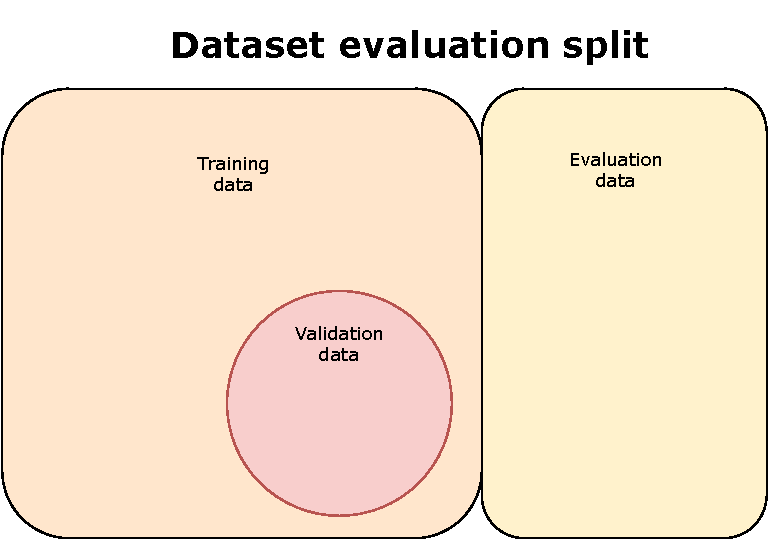
\includegraphics{img/train_test_data.pdf}
  \caption{Visualization of a dataset evaluation split. Training and evaluation data are subsets of the dataset, and the validation data is a subset of the training data.}
  \label{figure:dataset_train_test}
\end{figure}

It is common to split the inputs and output data into multiple parts, where some of the data is used to test the model. Testing of the model can happen at different times: after training sessions (evaluation) and in between epochs (validation). See figure \ref{figure:dataset_train_test} for a visual representation of a dataset evaluation split.

Before starting a model training session, we split the dataset into training and evaluation data, where the first part is what the model is trained to fit, and evaluation data is kept aside until the training is complete. Then we use it to check the performance of the trained model. Metrics used here is the value of the loss function (for example mean squared error) for value prediction, or classification metrics described in the previous subsection.

Validation data and is useful to include when we are developing the model, as we regularly see how the model is performing after each epoch. The metric used is usually the value of the loss function or the accuracy score, depending on the objective of the model. When the model is good enough for the desired task, we do not need validation data. We pass the validation split into the function that starts the model's training as either the validation\_split or the validation\_data parameter. If the validation\_split parameter is used (a number between 0 and 1), the validation data is calculated automatically before training starts. If, however, we want to use specific samples as validation data, we use the validation\_data parameter instead.

The function \textit{train\_test\_split} from the \textit{sklearn} package (see code \ref{code:sklearn_train_test_split}) is useful to split up the dataset into training and evaluation data. We input dataset (X, y), plus how large we want the training and test sets to be (number between 0 and 1, which determines the size of the test partition). The function also randomizes the data, preventing model to accidentally learn something correct for segments in a row that also are chronologically in order. After calling the function, you end up with two arrays for input data (\textit{X\_train, X\_test}), and two arrays for output data (\textit{y\_train, y\_test}). In this case the \textit{test\_size} is set to $0.4$, meaning that the test set contains $40\%$ of the total dataset and the remaining $60\%$ are in the training set.

\begin{figure}[h]
\begin{code}
    \begin{minted}[linenos]{python}
from sklearn.model_selection import train_test_split

X_train, X_test, y_train, y_test = train_test_split(X, y, 
                                                    test_size=0.4)
    \end{minted}
    \caption{Sklearn train and test split. After calling this function we end up with training and testing sets for both inputs and outputs.}
    \label{code:sklearn_train_test_split}
\end{code}
\end{figure}

\newpage

\subsubsection{Cross-validation}
\begin{figure}[h]
  \begin{code}    
      \begin{minted}[linenos]{python}
      from sklearn.model_selection import StratifiedKFold
  
      X, y = load_data(...)
  
      skf = StratifiedKFold(n_splits=3, shuffle=True)
  
      for train_index, test_index in skf.split(X, y):
          X_train, X_test = X[train_index], X[test_index]
          y_train, y_test = y[train_index], y[test_index]
  
          model = create_model(...)
          model.fit(X_train, y_train, ...)
          results = model.evaluate(X_test, y_test)
  
          # do something with results...
  
      \end{minted}
      \caption{StratifiedKFold from sklearn. The dataset is split in 3 parts (n\_splits on line 5), then training and evaluation happens for each of the parts.}
      \label{code:sklearn_k_fold}
  \end{code}
\end{figure}

\begin{figure}[!ht]
  \begin{center}
    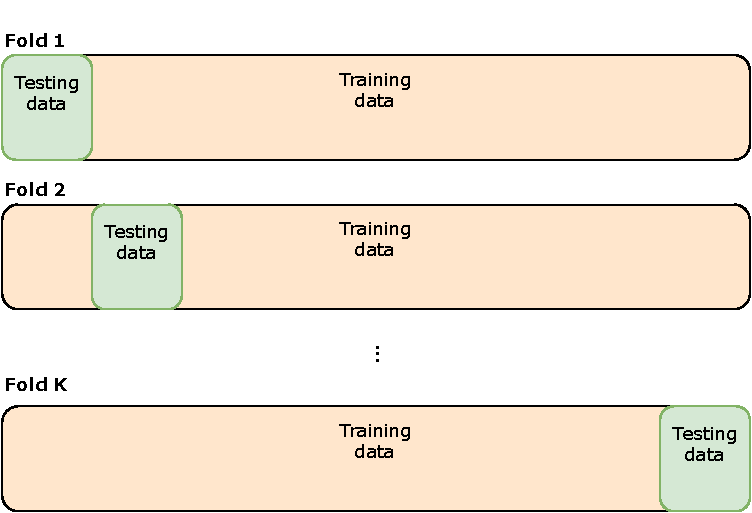
\includegraphics[height=8cm]{img/Cross-validation.pdf}
    \caption{K-fold cross-validation visualized. For each fold, a testing set is defined, and the rest of the data is a training set.}
    \label{figure:dataset_cross_val}
  \end{center}  
\end{figure}

Another popular choice is to use a technique called \textit{K-fold cross-validation}. It works by splitting the dataset into $K$ train and test sets, and for each of them, train the model on the training set and validate on the test set (visualized in figure \ref{figure:dataset_cross_val}). Cross-validation is a good way of checking if your model's performance truly is independent on which data samples it trained on. The higher number of splits ($K$) means fewer data samples to test on, so you need to keep that in mind (the same for \textit{train\_test\_split} if you set the \textit{test\_size} too low). Sklearn has an implementation of \textit{K-fold}, called \textit{StratifiedKFold}. An example of how it can be used is shown in code \ref{code:sklearn_k_fold}, where we perform a 3-fold cross-validation ($K = 3$). 

Performance testing of a model sometimes happens with both train/test-split and cross-validation. We set aside a small part of the dataset for evaluation and generating folds for the rest, then within each fold, we train and validate the model, and evaluate it against the part of the dataset that we set aside at the beginning. We note loss/accuracy scores for each fold and calculate the mean value which is the overall performance result.

Another way of using cross-validation to test the performance of a model is by leaving N participants out of the dataset. We do this by generating training data for the rest of the participants and evaluation data for the N participants left out. We log the performance scores for each fold, and then we find the overall average. 

In this thesis, we will use all described methods of splitting training and testing data. Simple train/test splitting is what we begin with during the development of the models. Then we perform cross-validation to verify that the models are consistent, and finally, we leave participants out one by one. The latter is essentially the same as 55-fold cross-validation, and it is a way of comparing our work to the work of Garcia-Ceja, E. et al., where they also evaluated their models by leaving participants out one by one \cite{GarciaCeja2018_classification_bipolar}. 


\section{Summary}
In this chapter, we introduced the general idea and flow of how the system detects the objectives of our goal, which for the first objective is visualized in figure \ref{figure:flow}. We presented the dataset in two parts, one containing demographic data and another one with motor activity measurements for each participant. Then, we described in detail how the data preprocessing algorithm works, which is responsible for translating the dataset into \textit{segments} we could input to the CNN, and \textit{labels} used for supervised learning. Finally, we introduced how we evaluate the performance of our CNN, in which we described the terminology of loss functions and optimizers, classification metrics, and training/testing data splits. 

Now that we have defined how everything around the CNN works, we can proceed to describe how we implemented the CNNs, which is the topic of the next chapter. 

\chapter{Implementation of Machine Learning Models}
\label{chapter:models}
The previous chapter showed that we structured the dataset into segments and labels so that we can apply supervised learning to it. The type of data in the dataset is activity measurements recorded from a smart-watch, which can have a high potential for analysis through ML. In this chapter, we provide a layer-by-layer description of how implemented our CNNs and linear regression model.

\section{Linear Regression}

Linear Regression is used a lot in statistics, where its primary purpose is to predict a target value based on independent predictors and is useful to find cause and effect relationships between variables \cite{linear_regression}. Before getting started on convolutional neural networks, we wanted to see if these problems were solvable with linear regression. The idea was to use the columns from the demographics dataset (see figure \ref{figure:demographics}). We did not expect high performance from this, as there are only 55 rows of participants. Anyone having a little bit of experience with machine learning will know that this is not nearly enough data. We wanted to do it regardless, to see how a linear regression model performed.

Not all of the columns are relevant, for example, \textbf{number} is unique for each participant, so it does not make sense to use. The column \textbf{melanch} also does not make sense to use, as there is only one participant with Melancholia. \textbf{Inpatient} cannot be used because the participants in the control group are not patients, and cannot be either inpatient or outpatient. The same goes for \textbf{edu}, \textbf{work} and \textbf{marriage}, but we do not have these data values for control group participants. We do not have their \textbf{afftype} or any of the \textbf{MADRS} scores either, but we already know them: \textbf{afftype} should be 0 (no depression) and both \textbf{MADRS} scores should be 0. 

We used the \textbf{afftype} column as a target in the regression. This way we could classify whether a participant is in the control or the condition group, by setting the \textbf{afftype} value to either 0 or 1 instead of 0, 1, 2 or 3 (values above 1 reduced to 1), and ran the regression on all of the remaining columns one by one:

\begin{itemize}
      \item \textbf{Gender}
      \item \textbf{Age}
      \item \textbf{Days}
      \item \textbf{MADRS1}
      \item \textbf{MADRS2}
\end{itemize}

The model for this task is straightforward. We created a sequential model (source code in appendix \ref{code:regression_model}) with one input layer and one output layer. The input is a dense layer which takes one value (the value of the current column), activates using \textit{relu} and outputs 5 neurons. In the output layer, we activate using a linear function (default activation function when none are specified) and return one value: the prediction. We compiled the model with the loss function \textit{Mean Squared Error} and the optimizer \textit{Adam}. 

Since we were predicting the \textbf{afftype} of a participant, which is a binary value (0 or 1) and a prediction from the model yields a value between 0 and 1, we rounded the prediction value to the nearest integer after running predictions on the test data. Doing it this way instead of making a classification model, makes the loss value more useful as a metric while training rather than accuracy. 

When testing the model, we wanted to achieve an accuracy of 100\% when using the \textbf{MADRS} scores. The task should be easy because of how easy it is using a simple check: if the MADRS score is 0, then the participant is in the control group. If not, the participant is in the condition group. We did not need to use machine learning on these columns but was interesting to train the model to find this relationship without telling it the simple rule. For the other columns, we did not know what to expect; maybe there was a relationship, maybe not.

\section{1D Convolutional Neural Network}

\subsection{Convolution}

\begin{figure}[h]
\begin{center}
    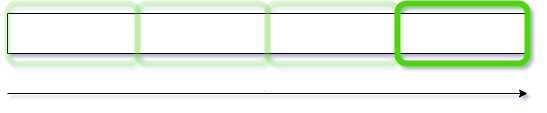
\includegraphics[height=2.5cm]{img/feature_detector.png}
    \caption{Feature Detector / Filter "sliding" over input data}
    \label{figure:feature_detector}
\end{center}
\end{figure}

\noindent The main ingredients in a CNN are \textit{convolutional} layers and \textit{pooling layers} \cite{deep_learning}. The convolutional layers are responsible for the convolution process, which in mathematics is a function derived from two given functions by integration which expresses how the shape of one is modified by the other \cite{convolution_definition}. 

The convolutional layer in machine learning consists of \textit{filters}, which are the sliding windows that go through the input data (see figure \ref{figure:feature_detector}). They are also called \textit{feature detectors}, and using 100 of them means that the layer can detect 100 features. The size of a filter is called \textit{kernel size}. The output of the convolutional layer is a matrix with one column for each filter, and one row for each step in the convolution. How many steps there are, is given by the length of the input data (also called \textit{height}) minus the kernel size plus 1.

\subsection{Creating the Model}
\begin{figure}[!ht]
\begin{center}
      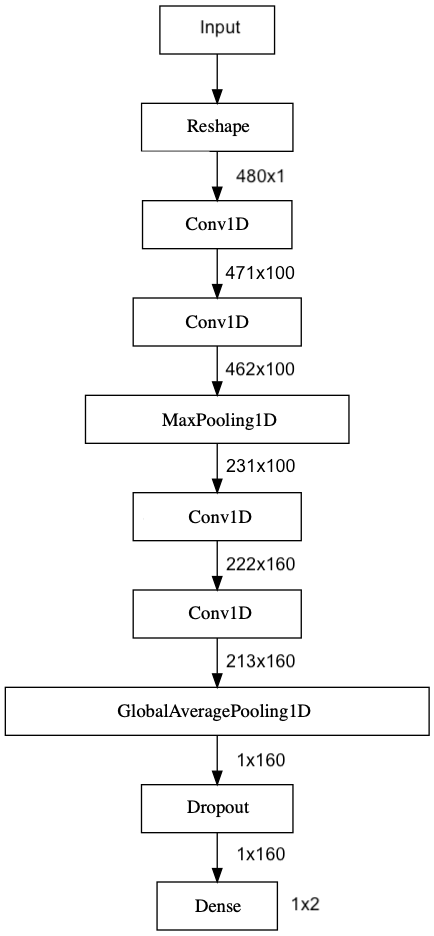
\includegraphics[height=19.5cm]{img/layers.png}
      \caption{The architecture of our convolutional neural network for the first objective. The segment length is 480 in this example. We can see the output shape underneath each layer.}
      \label{figure:layers}
\end{center}
\end{figure}

We built three CNN models. The models for the first two objectives were built for classification similarly, and for the third objective we came up with another model built for prediction. To make a CNN, we need some \textit{convolutional} and \textit{pooling} layers. Which layers added in between and the ordering of them, together with the parameters passed to the layers, is what makes the model perform differently. 

\subsubsection{Classification}
The following model was used to achieve our first two objectives; classifying whether a participant belongs to the \textbf{control} or \textbf{condition} group, and classifying the participant's \textbf{depression class}. The only difference between these two objectives is the number of classes we are trying to classify, and therefore only the output layer needs to be changed. Full source code can be found in the appendix (\ref{code:1d_conv_net_classifier}).

\begin{enumerate}
      \item We started by defining a \textbf{Sequential} model. This is easy to understand and readable way of defining a model. Alternatively, we could have used a \textbf{functional} model, which would give more control of inputs and outputs of the layers. A \textbf{functional} model would also be useful if we wanted to debug and optimize each layer within the model. 
      
      \item \textbf{Reshape}: In the first layer we needed to reshape the input data so that it becomes an $X$ by 1 matrix, where $X$ is the length of each segment. The reason for the reshape step is because the next layer (\textbf{Conv1D}) requires the input to contain the parameters \textit{batch, steps and channels}. \textit{Batch} will be set to \textbf{None}, \textit{steps} will be the segments, and \textit{channels} will be $1$ (because we only have one measurement value for each minute).
      
      \item \textbf{Conv1D}: This is the first \textit{convolutional} layer, where the required parameters are how many \textit{filters} wanted, and how big the \textit{kernel} should be. We used 100 filters and a kernel size of 10. Having less or more filters might have an impact on the performance, but we did not want to over-complicate the model yet. There are many different parameters that we can use on a layer like this, for example, \textit{padding} and \textit{strides}, but using the default values was a good choice for now. The output of this layer results in a $(X-10+1) \times 100$ matrix, where $X$ is the length of each segment here as well. The activation function for all convolutional layers in this model is \textit{ReLU} (Rectified Linear Unit). 

      \item \textbf{Conv1D}: The second convolutional layer looks exactly like the first one, and the output is a $(X-10+1-10+1) \times 100$ matrix. 
      \item \textbf{MaxPooling1D}: Pooling is important in a convolutional neural network to reduce complexity, and its role is to merge semantically similar features into one \cite{deep_learning}. 
            \textit{Max pooling} works by reducing to only the maximum value for each \textit{window} of size $N \times N$. We used 2 as 
            window size ($N$), resulting in matrix that is half the size of the input: $ \frac{X-10+1-10+1}{2} \times 100$. 
            Pooling may also help reduce \textit{overfitting}, which is when the model learns its training data too well and performs worse on unseen data.
      \item \textbf{Conv1D}: Two more convolutional layers were added, and after these, the input to the next layer will be a matrix of size
            $ \left( \frac{X-10+1-10+1}{2}-10+1-10+1 \right) \times 160 $.
      \item \textbf{GlobalAveragePooling1D}: Another type of pooling layer was added, which takes the average of weights within the network instead of the maximum.
            The output of the \textit{global average pooling} layer is a matrix of size $ 1 \times 160 $.
      \item \textbf{Dropout}: A dropout layer is used to reduce overfitting, by randomly ignoring units in the neural network \cite{dropout}. 
      \item \textbf{Dense}: The final layer in the model is a dense layer (fully connected) which reduces the matrix from $160$ values to 
            either $2$ or $3$ (for objective one and two), with the activation function \textbf{softmax}. 
            Then the output (a $1$ in one of the neurons) is mapped to the corresponding label.
\end{enumerate}

\subsubsection{Prediction}
To make the model work for our third objective, where we predicted the value of participant's MADRS score, we had to change a few layers. We removed two of the \textit{Conv1D} layers and applied the following after the global average pooling layer:

\begin{enumerate}
      \setcounter{enumi}{7}
      \item \textbf{Flatten}: The matrix was required to be flat (one dimensional) before proceeding to the final layers.
      \item \textbf{Dense}: A dense layer with $10$ neurons was added, with \textit{ReLU} as the activation function. 
      \item \textbf{Dense}: The output layer is a dense layer of size $1$, because we are predicting \textit{one} value. 
            Also, the activation function is \textit{linear} instead of \textit{softmax}.
\end{enumerate}

Source code for this model can also be found in the appendix (\ref{code:1d_conv_net_predictor}).

\section{Optimizing the models}

\noindent Out of the box, we did not think that the models were going to perform perfectly. Therefore we needed to experiment with each parameter that we passed to the models and find the best ones. We had some ideas of what to change:

\begin{itemize}
    \item Use different segment lengths
    \item Tweak hyper-parameters
\end{itemize}

\noindent The first idea, using different segment lengths, was the one we thought was going to impact the results the most. Having more data inside each segment will give the neural network more opportunities to learn features, and then be better at its job of either classifying or predicting the outcome. Having longer segments also means that each epoch of training would take more time because each layer has to process more data. In chapter \ref{chapter:training}, we describe the process of finding the optimal segment lengths for each objective.

Hyper-parameters are all the \textit{higher-order} parameters we compile/train the model with. These are the bells and whistles of the learning algorithm \cite{hyperparameters}, and they are different from the parameters learned by training the model and need to be fixed for one session of model training. Finding the perfect ones can be crucial for a well-performing model. Hyper-parameters that we use in our models include:

\begin{itemize}
      \item \textbf{Optimizer and learning rate}\\
          The \textbf{optimizer} function (as discussed earlier) is essential to lower the loss value when fitting the dataset to the model. 
          Different optimizers have different input parameters, and the \textit{learning rate} is one that all optimizers use. 
          Tweaking the learning rate can yield better results, but the default learning rate for the chosen optimizer is always a good starting point because it is what the author of the optimizer set as default.
      \item \textbf{Epochs}\\
          Defines how many iterations of training that are to be executed, and in most cases more epochs yield better results up to a certain point.
      \item \textbf{Batch size}\\
          This is how much data that is processed at the same time each epoch, and the best batch size to use can be completely different on two different models. 
      \item \textbf{Train/test split size}\\
          When building a neural network, we want as much data as possible to both train and to test on afterward. We cannot use all the data in both cases, so the most balanced split needs to be determined.
\end{itemize}

\section{Summary}
In this chapter, we explained how we implemented our linear regression and CNN models. We built a linear regression model able to train on one column in the demographics dataset at a time so that we could compare the performance afterward. Then, we built our one-dimensional CNNs for our primary objectives, explaining each layer and how the data flows through the network (output matrix shape for each layer). We described the main differences between our classification models and our MADRS prediction model. Finally, we defined how we wanted to optimize the CNN models after initial training. 

With our CNN models implemented, we can proceed to the next chapter, where we explain the training process for each of the models, including linear regression. We evaluate the performance of each model, and for the CNNs, we attempt to optimize hyper-parameters and the segment length. 

\chapter{Training the models}
\label{chapter:training}
For training deep neural networks, we often need expensive hardware if we want to do it on our own. The way to do it these days is to use cloud services such as Google or Amazon to run the ML once we have prepared the dataset and the model. We often pay for these services paid by the hour, but they are not expensive as long as we remember to shut them down after use, and only use them when we need to.

Our dataset, however, only contains 55 participants and only a few days of activity measurements for each participant, so using a service to train the model would not be necessary. We decided to train them on one of our personal computers, with an Nvidia GTX 1070 which should be enough in terms of performance.

This chapter is where we walk through the process of training the CNN and linear regression models. The performance of the models are evaluated, and we attempt to optimize them by tweaking the segment length and other hyper-parameters.
 
\section{Linear Regression}

\begin{figure}
\begin{center}
      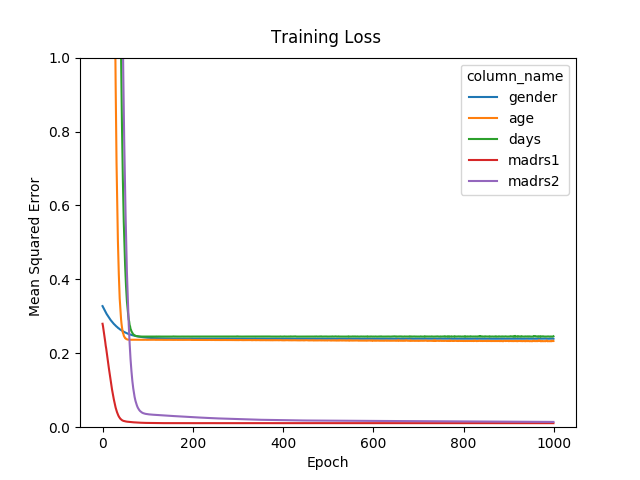
\includegraphics[height=9cm]{img/regression/results_kerasregressor_1k_epochs.png}
      \caption{Regression Training Loss (MSE) by Epoch. The MADRS scores of participants tell more about their condition than gender, age and days.}
      \label{figure:regression_training_loss}
\end{center}
\end{figure}

\begin{figure}
\begin{center}
      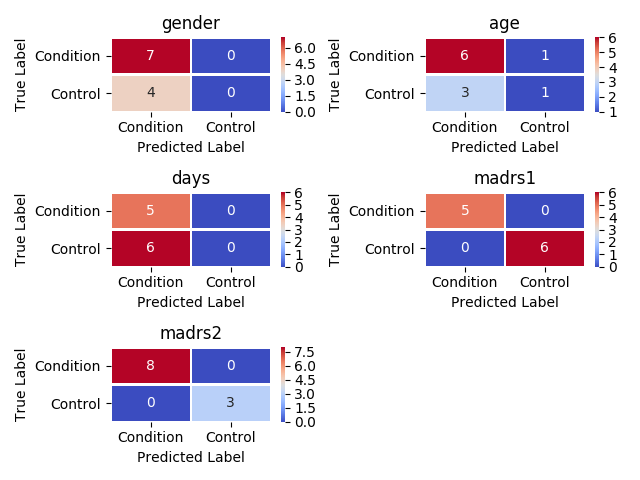
\includegraphics[height=12cm]{img/regression/confusion_kerasregressor_grouped.png}
      \caption{Confusion Matrices for Regression. For both MADRS1 and MADRS2, detections were perfect.}
      \label{figure:regression_test_confusion}
\end{center}
\end{figure}

We ended up training the regression model for 1000 epochs using a batch size of 16. Because of the simplicity of the model, a thousand epochs did not take that much time, and the training loss graph (figure \ref{figure:regression_training_loss}) shows that more epochs will not yield any better results. The loss does not reduce any more after the first 100 epochs for any of the columns. As we said earlier, we wanted the model to predict flawlessly based on the MADRS scores, and the loss results from training these are better than for the other columns. 

We used the \textbf{train\_test\_split} function to create training and testing data, and because of how few rows there are in this dataset, 
we used an 80/20 split for training and testing data. 20\% of the dataset in the test data seemed to be good enough for this experiment because we wanted to train on as many rows as possible. Note that the data elements that were in the test and train splits were different for each column. 

\subsection{Results}

The confusion matrices (figure \ref{figure:regression_test_confusion}) display the results when running the prediction on the test data (and then using them as classifications). We said we wanted 100\% on all metrics for the MADRS score columns, and this we can see that this is achieved because the model guessed everything right. The other columns have these performance scores (using \textbf{condition} as positive and \textbf{control} as negative):

\subsubsection{Accuracy}
$ A = \frac{TP+TN}{TP+TN+FN+FP} $
\\\\
- \textbf{Gender}: $\frac{7+0}{7+0+4+0} = 7/11 \approx 63\%$\\\\
- \textbf{Age}: $\frac{6+1}{6+1+3+1} = 7/11 \approx 63\%$\\\\
- \textbf{Days}: $\frac{5+0}{5+0+6+0} = 5/11 \approx 45\%$\\

\subsubsection{Precision}
$ P = \frac{TP}{TP+FP} $
\\\\
- \textbf{Gender}:$ \frac{7}{7+0} = 7/7 = 100\%$\\\\
- \textbf{Age}: $\frac{6}{6+1} = 6/7 \approx 86\%$\\\\
- \textbf{Days}: $\frac{5}{5+0} = 5/5 = 100\%$\\

\subsubsection{Recall}
$ R = \frac{TP}{TP+FN} $
\\\\
- \textbf{Gender}: $\frac{7}{7+4} = 7/11 \approx 63\%$\\\\
- \textbf{Age}: $\frac{6}{6+3} = 6/9 \approx 67\%$\\\\
- \textbf{Days}: $\frac{5}{5+6} = 5/11 \approx 45\%$

\subsubsection{Specificity}
$ S = \frac{TN}{TN+FP} $
\\\\
- \textbf{Gender}: $\frac{0}{0+0} = 0/0$\\\\
- \textbf{Age}: $\frac{1}{1+1} = 1/2 = 50\%$\\\\
- \textbf{Days}: $\frac{0}{0+0} = 0/0$\\

\subsubsection{F1 Score}
$ F1 = 2 \cdot \frac{P \cdot R}{P + R} $
\\\\
- \textbf{Gender}: $2 \cdot \frac{1 \cdot 0,63}{1 + 0,63} \approx 77\%$\\\\
- \textbf{Age}: $2 \cdot \frac{0,86 \cdot 0,67}{0,86 + 0,67} \approx 75\%$\\\\
- \textbf{Days}: $2 \cdot \frac{1 \cdot 0,45}{1 + 0,45} \approx 62\%$\\

Looking away from the results of \textbf{madrs1} and \textbf{madrs2}, the performance scores tell us that the model is good at predicting that someone is in the condition group (precision). Other than that, we cannot learn that much from them. Also, we have undefined specificity for both gender and days because we do not have any predictions for the values required to calculate them. 

However, we learned a lot about ML and linear regression doing this experiment, and we looked at it more like a warmup for the more complex models that we built for the next objectives.

\section{1D CNN: Control vs Condition groups}

\subsection{Training and finding the optimal segment length}

Next up was our objective to classify whether a participant belongs to the control group or the condition group. As we said in the section about optimizing the model, the segment length is what we thought was going to impact the result the most. To test this theory, we trained the model to fit input data created with segment lengths of 1, 2, 4, 8, 16, 24, 48 and 96 hours. 

The input data was split using \textbf{train\_test\_split} so that the training data was 80\% of the total and the rest was going to be used for testing after the training was complete. We used 40\% the training data as validation data, which made it easy for us to tell if the model was learning from epoch to epoch or not. 

We did the training for each of the eight different input sets for ten epochs. We used a batch size of 16 and the Adam optimizer with a default learning rate of 0,001 throughout this experiment. The primary goal here was to find the best segment length to use, and not to train the models to be perfect, so these hyper-parameters seemed fine for this purpose. Our guess before we started with the experiment was that the more hours of data we used, the better, meaning that 96 hours of data in each segment was going to give us the best model (from what was possible with only ten epochs).

Looking at the training history graphs (figure \ref{figure:control_condition_10e_train}) for how the training went epoch by epoch, we noticed that the results were better when increasing the number of hours up to 48, and then it did not seem to be any better for 96 hours. This was the case for both training and testing, as the evaluation graphs (results after testing the model with the test-split - figure \ref{figure:control_condition_10e_eval}) also show straight lines from 48 hours to 96 hours. The question was whether 48 hours was our optimal length, or if we just needed to train it more.

To find the best segment length, we needed to experiment with more epochs. We reran the same experiment for 50 epochs, with 48, 72 and 96 hour long segments. However, from the training graph (figure \ref{figure:control_condition_50e_train}), we can see that nothing more was achieved with segments longer than 48 hours. 

The evaluation data classifications from the model trained to fit 48-hour segments seen in the confusion matrix (figure \ref{figure:control_condition_confusion_matrix_48h}) are close to perfect. The additional 40 epochs of training reduced the false negative classifications by a little bit, which was worth the time in our opinion as we want the value of wrong classifications to be as close to 0 as possible. The model scored above 0.99 on all classification performance metrics (table \ref{table:control_condition_performance}), which is promising.

\begin{figure}
\begin{center}
      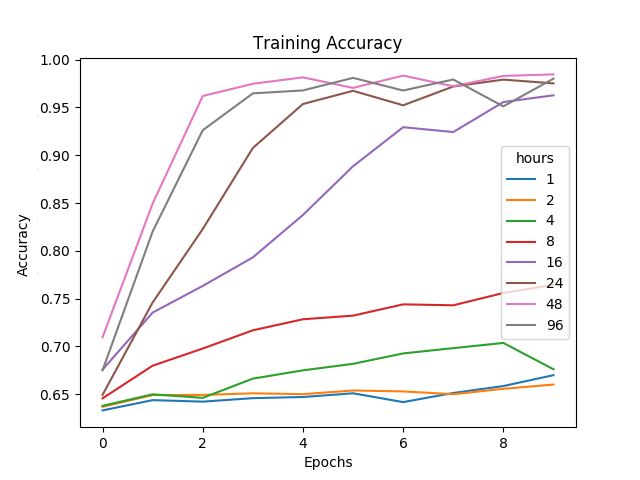
\includegraphics[height=10cm]{img/control_condition/plot_acc_train.png}
      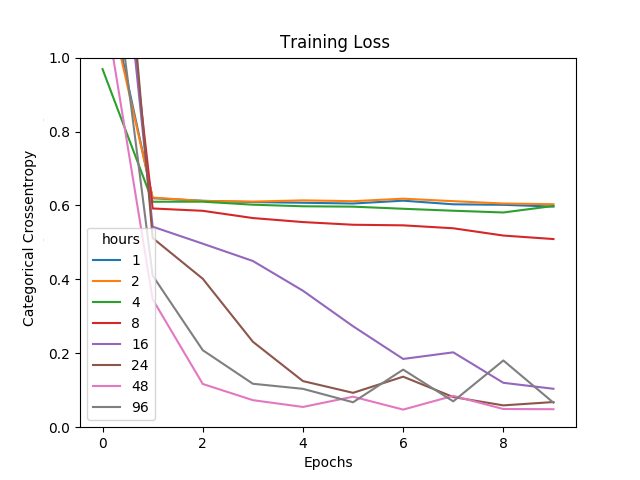
\includegraphics[height=10cm]{img/control_condition/plot_loss_train.png}

      \caption{Graphs for training loss and accuracy, where we can see the model's performance for different segment lengths throughout 10 epochs of training.}
      \label{figure:control_condition_10e_train}
\end{center}
\end{figure}

\begin{figure}
\begin{center}
      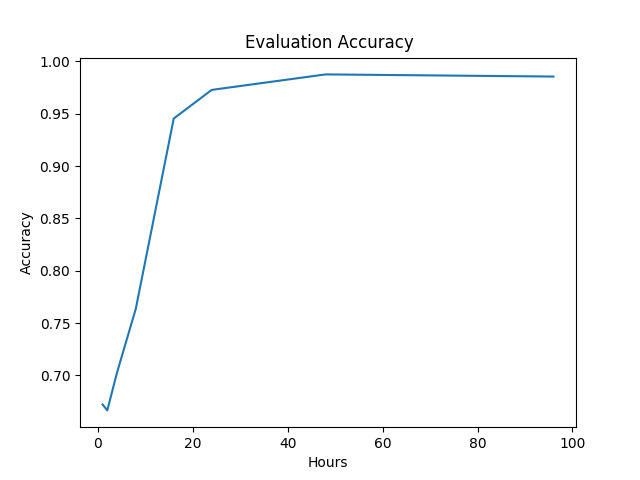
\includegraphics[height=10cm]{img/control_condition/plot_acc_eval.png}
      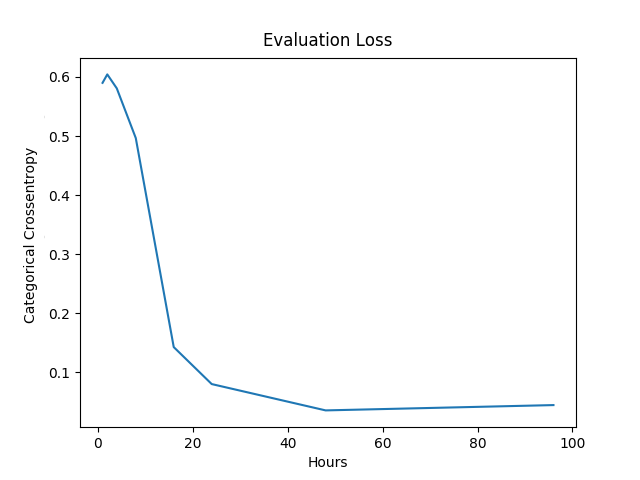
\includegraphics[height=10cm]{img/control_condition/plot_loss_eval.png}

      \caption{Evaluation loss and accuracy. We can see how the model performed when tested against evaluation data. The performance did not seem to improve with segments longer than 48 hours.}
      \label{figure:control_condition_10e_eval}
\end{center}
\end{figure}

\begin{figure}
\begin{center}
      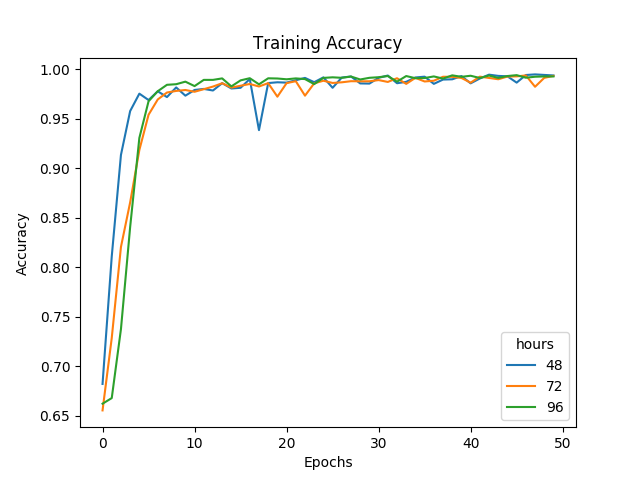
\includegraphics[height=10cm]{img/control_condition/plot_acc_train_50e.png}
      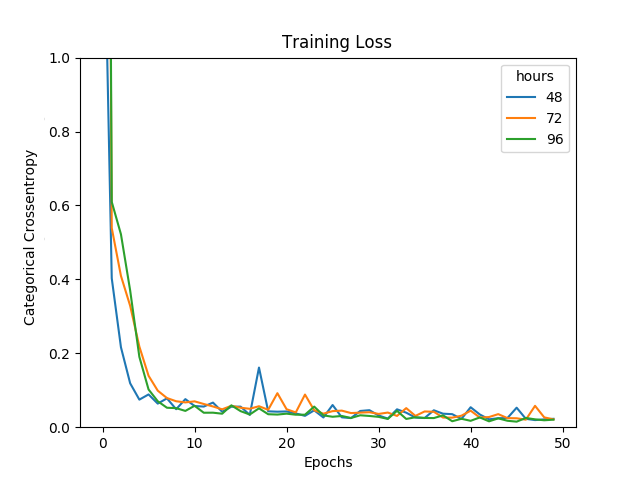
\includegraphics[height=10cm]{img/control_condition/plot_loss_train_50e.png}

      \caption{Graphs for training loss and accuracy, where we can see the model's performance for different segment lengths throughout 50 epochs of training. Using 48 hours long segments was still the best option (performance did not improve much for longer segments).}
      \label{figure:control_condition_50e_train}
\end{center}
\end{figure}

\begin{figure}
\begin{center}
      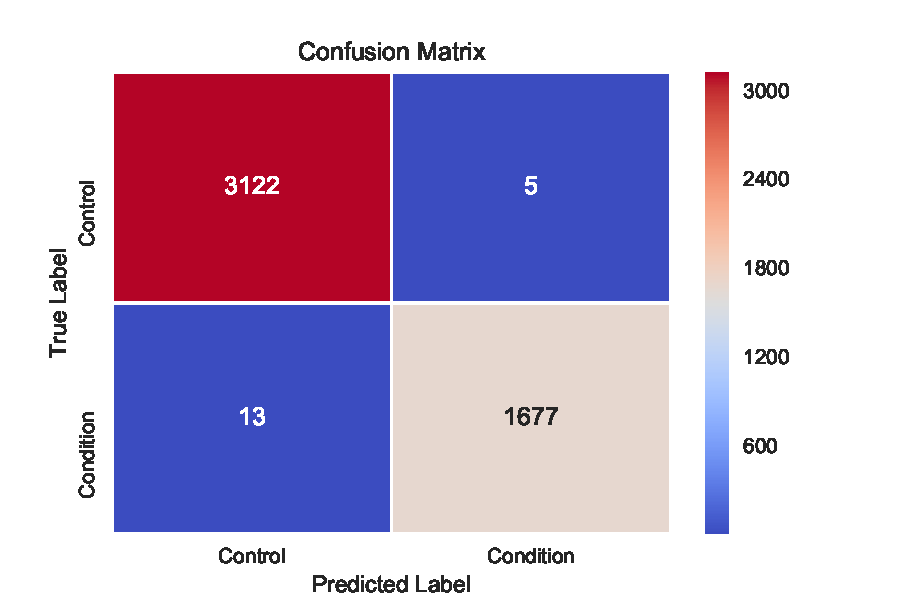
\includegraphics[height=8cm]{img/control_condition/50ep.pdf}
      \caption{Confusion matrix for testing the classifier on unseen data. After training the model for 50 epochs, it was able to correctly classify 3122 control group and 1677 condition group segments.}
      \label{figure:control_condition_confusion_matrix_48h}
\end{center}
\end{figure}

%TP   FN   
%FP   TN

\begin{table}[h]
\begin{center}
      \begin{tabular}{|l|l|l|l|l|}
            \hline
            \bfseries Accuracy & \bfseries Precision & \bfseries Recall & \bfseries Specificity & \bfseries F1 \\\hline
            0.996 & 0.996 & 0.998 & 0.992 & 0.997 \\\hline
      \end{tabular}
      \caption{Performance metrics for control vs condition group classifier.}
      \label{table:control_condition_performance}
\end{center}
\end{table}

\vfill

\subsection{Cross-validation}

To ensure that our model is not overfitting and did not get lucky when classifying the samples from the testing set, we proceeded to use 3-fold cross-validation. First, we split the dataset in two like before, into a train and test set (80/20 split here as well). Then we generated three folds containing training and validation parts, where for each fold a model was trained to fit the inputs. Each epoch the model was validated against the validation split. After training a model for a fold, we evaluated them by looking at the mean accuracy/loss against the global test split. If the accuracy was still high and the loss was still low, the model would have a good chance of doing correct classifications on unseen data.

\begin{table}[h]
      \begin{center}
          \begin{tabular}{|l|l|l|}
              \hline
              \bfseries Fold & \bfseries Loss & \bfseries Accuracy
              \csvreader[head to column names]{code/logs/control_vs_condition/5f_cv.csv}{}
              {\\\hline\fold & \loss & \accuracy}
              \\\hline
              \bfseries Mean & \bfseries 0.063 & \bfseries 0.98
              \\\hline
          \end{tabular}
          \caption{3-Fold Cross validation. Mean accuracy was 0.98 and mean loss was 0.06.}
          \label{table:control_condition_5f_cv}
      \end{center}
\end{table}

To make this process quick, we trained the model for each fold only for ten epochs. The goal was to prove consistency in the model and not achieve high performance, so it seemed enough. As one can see in the cross-validation results (table \ref{table:control_condition_5f_cv}), we have a mean loss of $0.06$ and a mean accuracy of $0.98$, which means that the model is consistently correct in most classifications.

\subsection{Leaving one participant out}

However, the above results were for each segment and label, and not specific to any participant. Even though we reduced the chance of overfitting by keeping aside randomized training and testing data, there is a high chance that the training data contains samples from all participants. Garcia-Ceja, E. et al. did \textit{leave one participant out validation} in their paper \cite{GarciaCeja2018_classification_bipolar}, which means that for each participant in the dataset, keep them outside the training data, train on the rest of the participants, then make predictions on the participant that was left out. Each prediction for the left out participant can be different, so to determine the final label they used majority voting (using the most common predicted label). 

We proceeded to do the same experiment as Garcia-Ceja, E. et al., as it would be a good way of comparing our work. For each participant, we generated input data that did not contain any activity data from the participant. Then we created a model and trained it to fit the input data for ten epochs (any more would take too much time considering we had to train 55 models), and made predictions using majority voting. 

\begin{figure}[h]
\begin{center}
      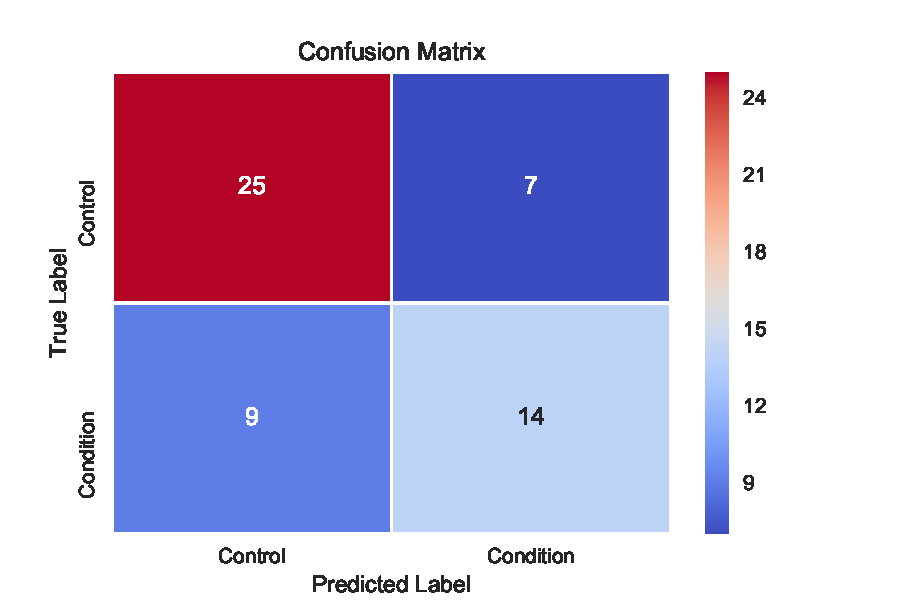
\includegraphics[height=8cm]{img/control_condition/leave_one_out.pdf}
      \caption{Confusion matrix containing detected classes after leave one participant out experiment. The model was best at classifying participants in the control group.}
      \label{figure:control_condition_conf_loo}
\end{center}
\end{figure}

\begin{table}[h]
\begin{center}
      \begin{tabular}{|l|l|l|l|l|l|}
            \hline
            \bfseries Label & \bfseries Accuracy & \bfseries Precision & \bfseries Recall & \bfseries Specificity & \bfseries F1 \\\hline
            Control & 0.71 & 0.74 & 0.78 & 0.61 & 0.76 \\\hline
            Condition & 0.71 & 0.67 & 0.61 & 0.78 & 0.64 \\\hline
            \bfseries Mean & \bfseries 0.71 & \bfseries 0.71 & \bfseries 0.70 & \bfseries 0.70 & \bfseries 0.70 \\\hline
      \end{tabular}
      \caption{Performance metrics for leave one participant out experiment.}
      \label{table:control_condition_performance_loo}
\end{center}
\end{table}

Earlier results were almost perfect, so we expected the results of this experiment to be better than what we can see in the confusion matrix (figure \ref{figure:control_condition_conf_loo}). The model did an excellent job of detecting true negatives (where the correct label and the predicted label is \textit{control}, but the number of false positives and false negatives were a bit too high. We could train the models for more than ten epochs and hope for better results, but we assume it would not be much better because of how little training loss and accuracy changed after the first ten epochs (as seen in the training graph - figure \ref{figure:control_condition_50e_train}). 

\section{1D CNN: Depression Classes}

\begin{figure}[!ht]
      \centering
      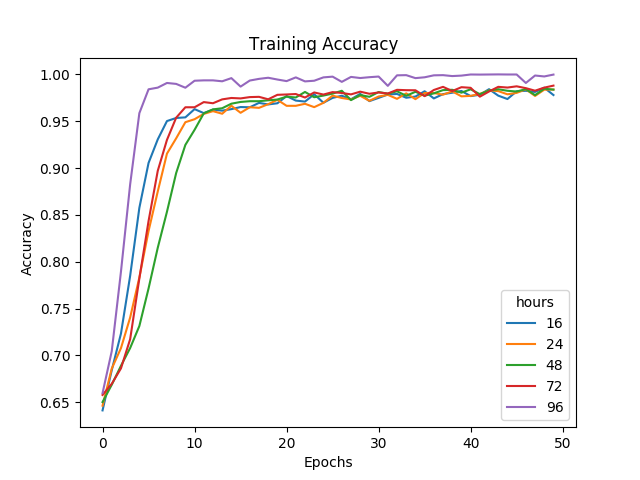
\includegraphics[height=10cm]{img/depression_class/plot_acc_train.png}
      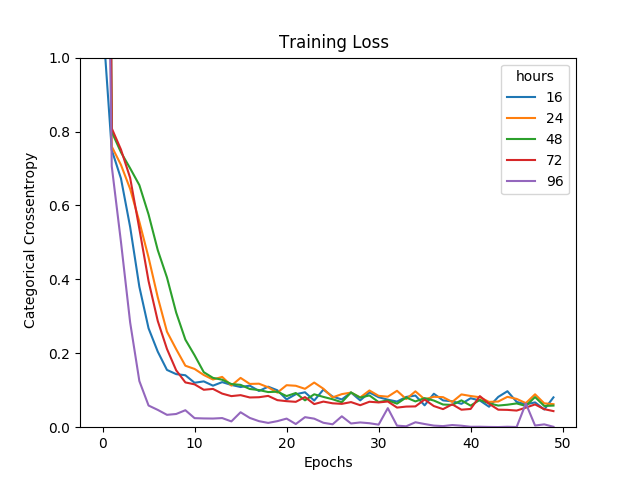
\includegraphics[height=10cm]{img/depression_class/plot_loss_train.png}

      \caption{Training loss and accuracy for different segment lengths. After 50 epochs we can see that loss and accuracy continues to be better with longer segments.}
      \label{figure:depression_class_50e}
\end{figure}

\begin{figure}[!ht]
      \centering
      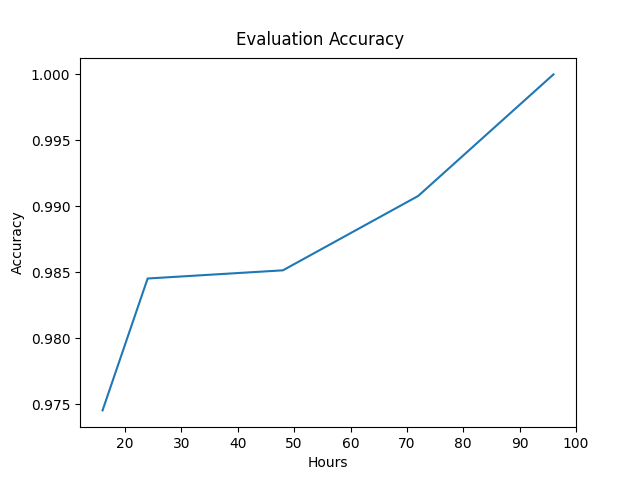
\includegraphics[height=10cm]{img/depression_class/plot_acc_eval.png}
      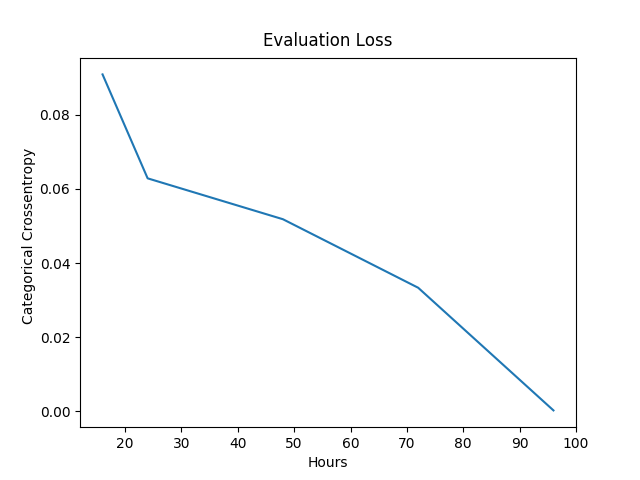
\includegraphics[height=10cm]{img/depression_class/plot_loss_eval.png}
      \caption{Evaluation loss and accuracy for different segment lengths. Unlike for the first objective, we continue to gain performance when increasing the segment length.}
      \label{figure:depression_class_50e_eval}
\end{figure}

\begin{figure}
\begin{center}
      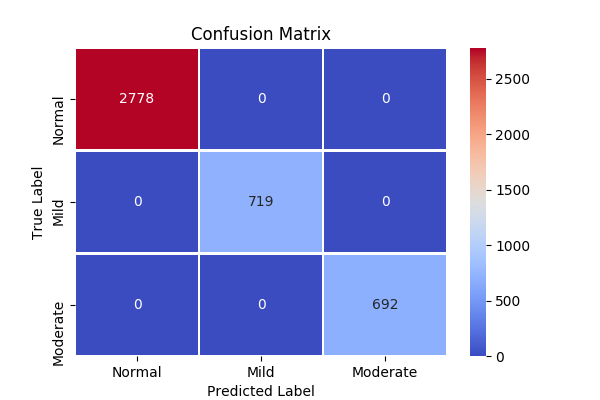
\includegraphics[height=8cm]{img/depression_class/conf_5760_60_50_32.png}
      \caption{After training the model on 96 hour long segments for 50 epochs, classification on test-data segments is perfect.}
      \label{figure:depression_class_confusion_matrix_96h}
\end{center}
\end{figure}

\subsection{Training and finding the optimal segment length}

The next neural network we trained was for classifying how depressed the participants were. Depression classes are, as we said before, 
based on their MADRS score which is 0 for participants in the control group and differs between 11 and 28 in the condition group (figure \ref{figure:demographics}). We labeled participants with MADRS score 0 as not depressed, between 11 and 19 as mildly depressed, and above 20 as moderately depressed. 

Using what we previously discovered from classifying control vs. condition groups, we knew how we wanted to satisfy this objective. First, find the optimal segment length, then use the best segment length in cross-validation, and guarantee that the performance is consistent. 

In the previous experiment, there was a clear threshold after segment lengths of 24 hours where the performance did not improve that much if increased more (figure \ref{figure:control_condition_10e_train}). The results were just a little bit better for 48 than 24 hours and worse for longer segments. The question was whether the threshold existed for depression classes also, or if we could use longer segments to achieve better results.

We experimented the same way as before, except that we went straight for 50 epochs and skipped the shortest segments of 1, 2, 4 and 8 hours, as we were positive these segments would not be any good. We proceeded to train segment lengths of 16, 24, 48, 72 and 96 hours. Looking at the training and testing graphs (figure \ref{figure:depression_class_50e}), we can see that the results for 96-hour segments were outstanding. We achieved an accuracy of 100\% on the testing set. The confusion matrix (figure \ref{figure:depression_class_confusion_matrix_96h}) shows not a single error in classification. 
 
\subsection{Cross-validation}

\begin{table}[h]
\begin{center}
      \begin{tabular}{|l|l|l|}
            \hline
            \bfseries Fold & \bfseries Loss & \bfseries Accuracy
            \csvreader[head to column names]{code/logs/depression_class/cv.csv}{}
            {\\\hline\fold & \loss & \accuracy}
            \\\hline
            \bfseries Mean & \bfseries 0.033 & \bfseries 0.991
            \\\hline
      \end{tabular}
      \caption{3-Fold Cross validation for this experiment to verify consistency of the model. All three folds perform well.}
      \label{table:depression_class_cv}
\end{center}
\end{table}

To make sure this was not just lucky, we needed to cross-validate here as well. We split the dataset into a training and testing set (80\%/20\%), then did three-fold cross-validation on the training set, just as before. If all three folds had similar accuracy and loss, and the mean values were good (close to 1.0 for accuracy and close to zero for loss), we had achieved a consistent model, and the model would be fit perfectly, at least for the 55 participants in the dataset. 

We trained the three models for 15 epochs each. We knew that was not enough to give us 1.0 accuracy (need around 50 epochs for that), but we aimed for somewhere around 0.98-0.99 for all folds. Looking at the cross-validation results (table \ref{table:depression_class_cv}), we can see that the lowest accuracy was 0.985 and the highest was 0.998. The mean accuracy for all three folds was 0.99, which is what we wanted to see. 

\subsection{Leaving one participant out}

\begin{figure}[h]
\begin{center}
      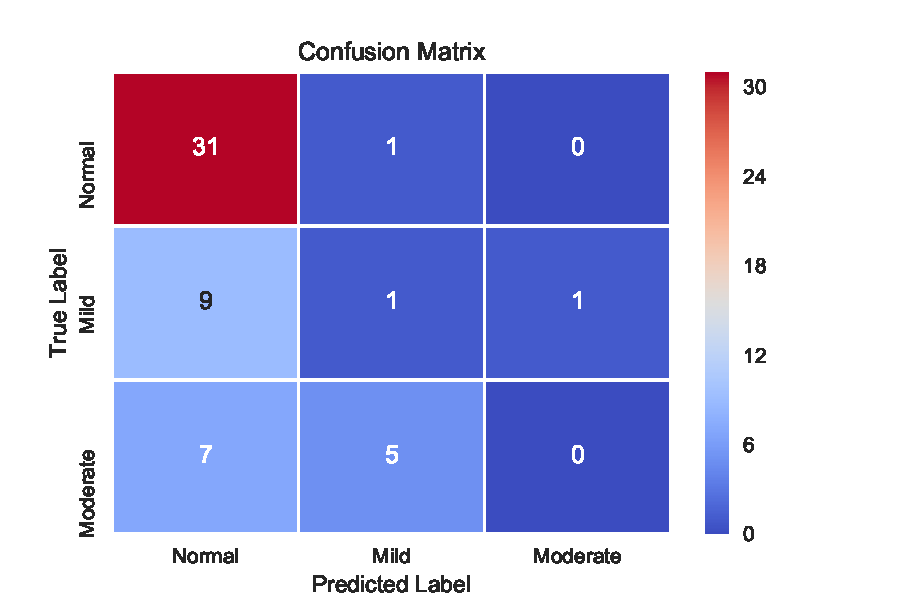
\includegraphics[height=8cm]{img/depression_class/leave_one_out.pdf}
      \caption{Confusion matrix containing detected classes after leave one participant out experiment. The model was only good for detecting normal participants.}
      \label{figure:depression_class_conf_loo}
\end{center}
\end{figure}

\begin{table}[h]
\begin{center}
      \begin{tabular}{|l|l|l|l|l|l|}
            \hline
            \bfseries Label & \bfseries Accuracy & \bfseries Precision & \bfseries Recall & \bfseries Specificity & \bfseries F1 \\\hline
            Normal & 0.69 & 0.66 & 0.97 & 0.30 & 0.79 \\\hline
            Mild & 0.70 & 0.14 & 0.09 & 0.86 & 0.11 \\\hline
            Moderate & 0.76 & 0.0 & 0.0 & 0.98 &  \\\hline
            \bfseries Mean & \bfseries 0.72 & \bfseries 0.30 & \bfseries 0.35 & \bfseries 0.71 & \bfseries 0.30 \\\hline
      \end{tabular}
      \caption{Performance metrics for leave one participant out experiment.}
      \label{table:depression_class_performance_loo}
\end{center}
\end{table}
We repeated the same experiment from the end of the previous objective, where we trained on all participants except one that we left for testing afterward. Looking at the confusion matrix (figure \ref{figure:depression_class_conf_loo}), the model seemed to be good at detecting non-depressed participants (F1-score of 0.79), and terrible at everything else (F1-score of 0.11 for mild depression and the model did not detect any participant with moderate depression). Overall, we calculated a mean F1-score of 0.30 for this model (see table \ref{table:depression_class_performance_loo}). 


\section{1D CNN: MADRS Score Prediction}
Now that we have models for classifying both whether a participant belongs to the control group or the condition group and how depressed participants are, we can get started on our last objective which is predicting the MADRS score of our participants. 

Training a prediction model is significantly more computationally heavy than training a classification model. We noticed this as soon as we started the training when the loss started on around 100 which is very high, and prediction on test data after a few epochs was poor. In classification, we were used to training and validation loss between 1 and 0 and reaching a high accuracy after only a few epochs. We had to train for some epochs to compare segment lengths, which would only show which are best in the first epochs.

\subsection{Segment length}
The plan was to perform 100 epochs of training for different segment lengths. We used the same segment lengths as we did for the previous model: 16, 24, 48, 72 and 96 hours. Since the two classification experiments had a different optimal segment length, it was an interesting question whether this was the case for MADRS prediction as well. 

After finding the best segment length, we used the one with the most promising results to train the model for a more extended period. We wanted to see how good performance we could achieve if we increased the number of epochs by a lot and let it learn overnight. 

\subsection{Cross-validation}
Before training the model to be as perfect as possible, we did cross-validation to check its consistency. Just as we had done before, we performed 3-fold cross-validation. For each fold, we trained the model for 100 epochs to fit the corresponding training data and validated on the corresponding validation data. Then, after a model had completed its training, it was evaluated against the global test data (same procedure as the two previous experiments). Finally, the Mean Squared Error for each fold was saved and compared with other folds to see how they averaged. 

\begin{table}
\begin{center}
      \begin{tabular}{|l|l|l|}
            \hline
            \bfseries Fold & \bfseries Mean Squared Error
            \csvreader[head to column names]{code/logs/madrs_prediction/cv.csv}{}
            {\\\hline\fold & \mse}
            \\\hline
            \bfseries Mean & \bfseries 31.40
            \\\hline
      \end{tabular}
      \caption{3-Fold Cross validation for the prediction model. Only small variation between the folds tells us that the model is consistent enough.}
      \label{table:madrs_prediction_cv}
\end{center}
\end{table}

\begin{figure}
      \centering
      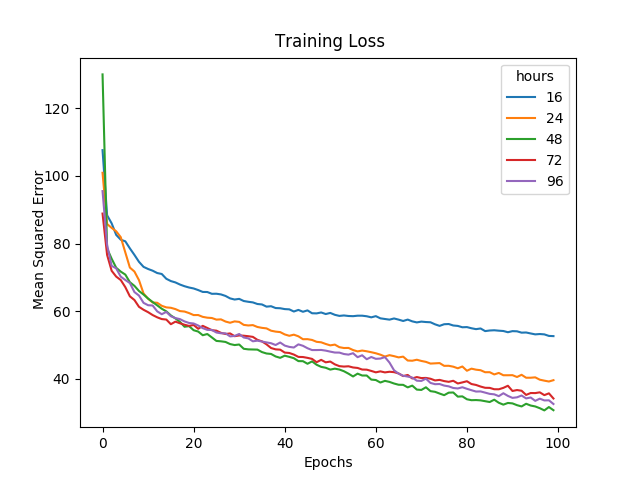
\includegraphics[height=10cm]{img/madrs_prediction/plot_loss_train.png}
      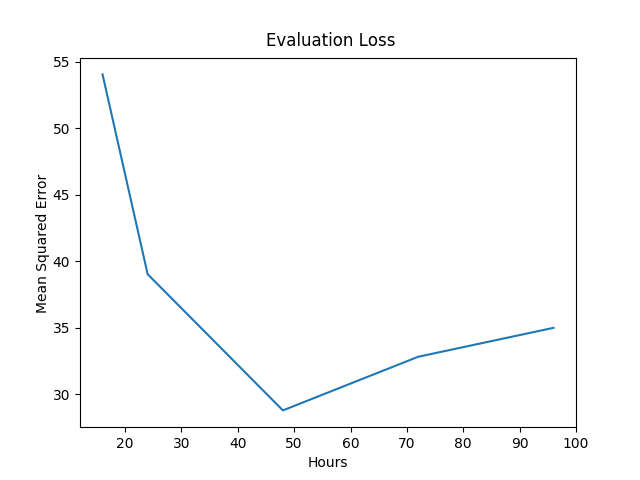
\includegraphics[height=10cm]{img/madrs_prediction/plot_loss_eval.png}

      \caption{Training the MADRS prediction model for 100 epochs with different segment lengths. The model trained on 48-hour segments performed best.}
      \label{figure:madrs_prediction_50e}
\end{figure}

\subsection{Hyper-parameters}
\begin{figure}
\begin{center}
      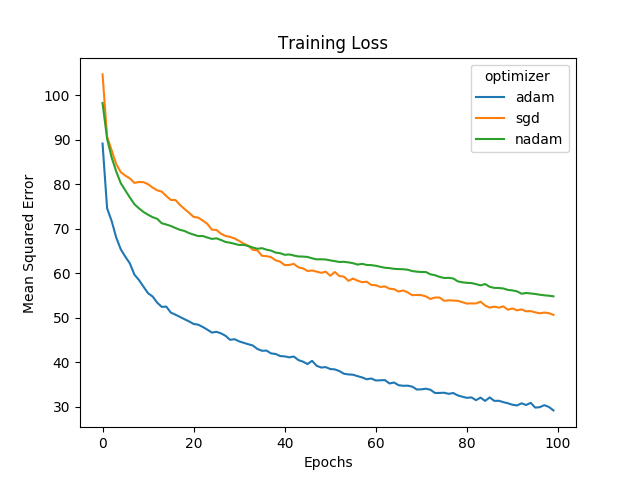
\includegraphics[height=8cm]{img/madrs_prediction/optimizers.png}
      \caption{Training the models with 48-hour segments for 100 epochs, comparing different optimizers. The Adam optimizer performed significantly better than SGD and Nadam.}
      \label{figure:madrs_prediction_optimizers}
\end{center}
\end{figure}

\noindent From the training and evaluation graphs (figure \ref{figure:madrs_prediction_50e}), it seemed like the best was to use 48-hour segments. We do not know what is best for training 
the model further, but this was what we settled on using. 

Also, unlike the classification experiments, we experimented more with hyper-parameters. The Adam optimizer with default learning rate did the job for classification, 
but now that we had to train for thousands of epochs, these parameters had the potential to affect the results by a lot. 
We proceeded to compare three different optimizers: Adam, SGD, and Nadam. We had to change the learning rate to get SGD to work 
(the default which is 0.01 \cite{keras_docs} resulted in NAN MSE for some reason). All optimizers were set to use a learning rate of 0.0001. 
The optimizer comparison graph (figure \ref{figure:madrs_prediction_optimizers}) shows that Adam was the best choice for MADRS prediction as well. 


\subsection{Training the model}
To summarize, this model was trained to fit segments of length 48 hours (2880 minutes). It was trained with the optimizer Adam using a learning rate of 0.0001. We did not change the batch size; we kept this at 16. We split the dataset into 60\% training data and 40\% testing data. Based on the time it took to train each of the 100-epoch experiments, we calculated that around 2700 epochs of training would be a realistic amount.

When we checked for results the next day, we could see the training had resulted in a mean squared error approximately at 4.0 (on validation data). The training graph (figure \ref{figure:madrs_prediction_history}) shows that further training would not necessarily give any better results. Predictions on the test data (figure \ref{figure:madrs_prediction_testset}) looked very promising. The graph shows correct MADRS scores in the x-axis and the predicted MADRS scores in the y-axis. Each blue dot is a prediction, and the dotted black line is a linear guideline for the perfect predictions (where the predicted and correct scores are the same). 

\begin{figure}
\begin{center}
      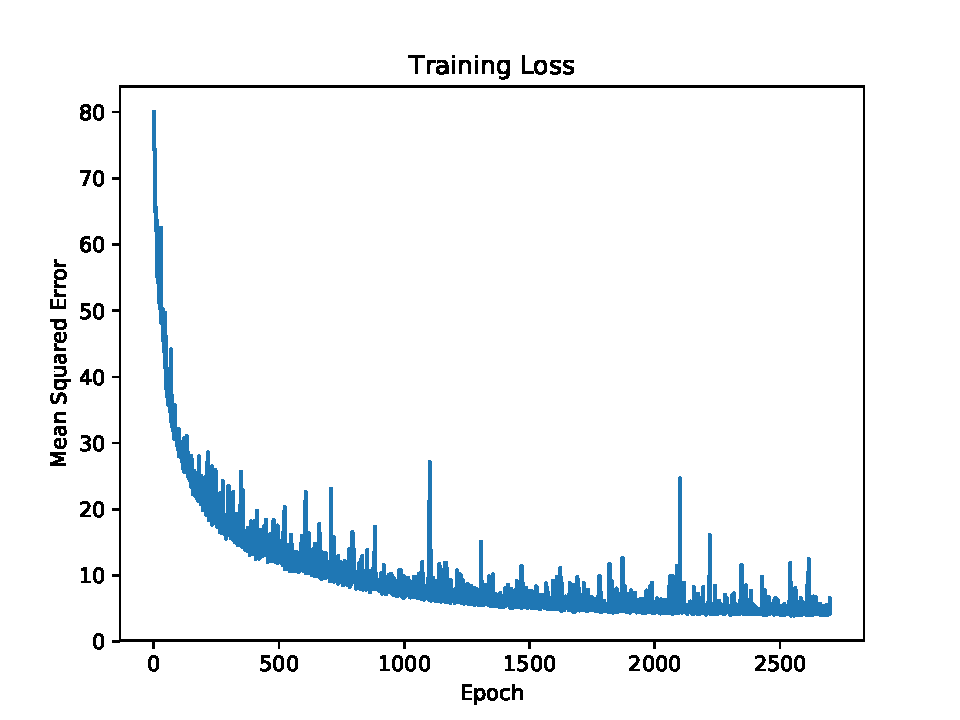
\includegraphics[height=8cm]{img/madrs_prediction/train_history.pdf}
      \caption{MADRS Prediction: Training history throughout 2700 epochs. The MSE is approximately 4.0 after 2000 epochs.}
      \label{figure:madrs_prediction_history}
\end{center}
\end{figure}

\begin{figure}
\begin{center}
      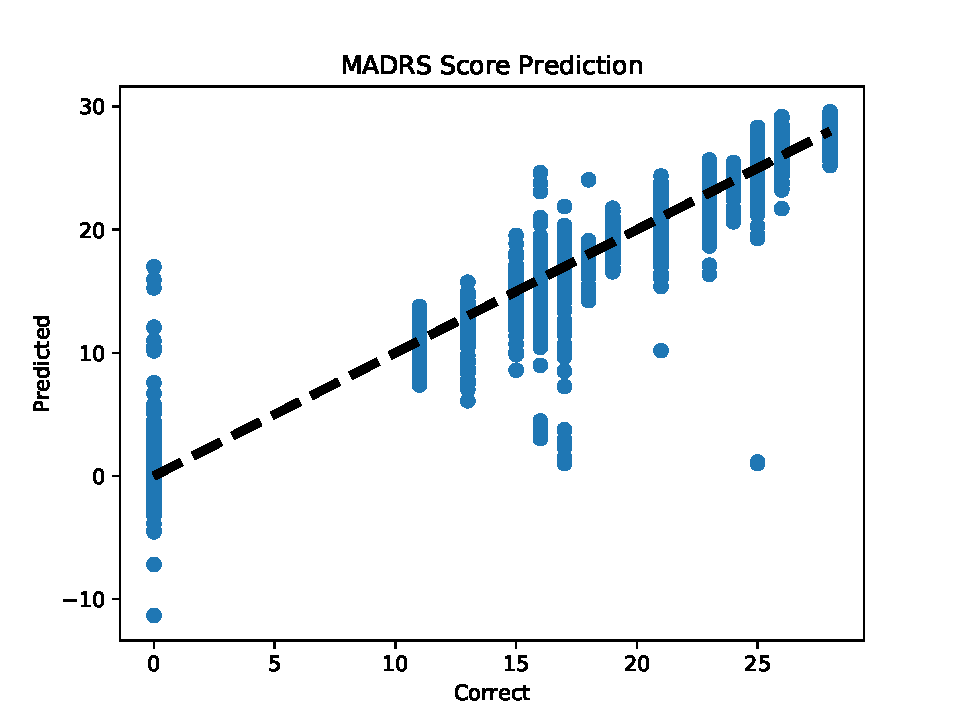
\includegraphics[height=8cm]{img/madrs_prediction/predictions.pdf}
      \caption{Running the MADRS prediction model on unseen segments. The predictions are not perfect, but they somewhat follow the line where predictions and correct MADRS scores are the same.}
      \label{figure:madrs_prediction_testset}
\end{center}
\end{figure}
\newpage

\section{Summary}
In this chapter, we have presented how we trained each of our ML models. With linear regression, we got the model to detect with 1.0 accuracy whether participants are depressed or not when training on the madrs1 and madrs2 values. We did not learn much from training on other columns from the demographic dataset, other than the fact that the model was good at detecting that participants were depressed when it was also the correct label (precision).

From the CNN detecting control/condition groups, we learned that 48-hour long segments (2880 minutes) resulted in the highest performance with an F1-score of 0.997 when evaluated against the test-split of the dataset. \textit{Leave one participant out} evaluation resulted in an F1-score of 0.70. The difference between the performance before and after this type of evaluation is a topic for the discussion in the next chapter. 

The optimal segment length was different for the CNN that detects depression classes. We achieved 1.0 evaluation accuracy after 50 epochs of training on segments of length 96 hours (5760 minutes). However, in with the \textit{leave one participant out experiment}, we achieved only an average accuracy of 0.72 and F1-score of 0.30. 

MADRS score prediction happened with a different CNN model, but it was similar to the first objective when it came to the optimal segment length of 48 hours. For this model, we also compared optimizers, finding that Adam was the best choice. We achieved a validation and evaluation loss (MSE) of approximately 4.0 after training the model. 

\part{Conclusion}
\chapter{Discussion}
\label{chapter:discussion}
\section{Convolutional neural networks for mental health detection}
We have evaluated how CNNs performed on motor activity measurements from bipolar and unipolar depressed patients (condition group) together with non-depressed control participants. We completed our objectives of creating classification models for detecting whether a participant belongs to the control group or the condition group, the depression class of a participant (not depressed, mild depression or moderately depressed), and finally a prediction model for estimating the MADRS score of participants. 

We did not leave one participant out on the last model, because it had to be trained for at least 1500 epochs before the mean squared error was acceptable (see figure \ref{figure:madrs_prediction_history}). Training took several hours, and multiplying that with 55 (one training session for each participant), the experiment would take days. We consider this to be a weakness in our work and it makes the MADRS prediction model less trustworthy. 

\subsection{Limited number participants}
The dataset consists of only 55 participants, which is very limited. It was a good set of data for us in our thesis, but in order to use it in the real world, more participants is a requirement. Measurements from more people and different ethnicities and age groups around the world would significantly increase the viability of the dataset. We suggest collecting more data before applying this research anywhere in the real world.
 
We think that the number of participants is the main issue that made the classifier only decent when leaving one participant out. The difference between people is far too big for our CNNs to handle with a dataset containing such few participants. We divided the participants into control/condition group. The condition group itself contains participants who suffer from one type of depression, regardless of which type of bipolar disorder (or unipolar depressed) they are diagnosed with. With data from more people, the network could potentially pick up and learn more similarities between people within the same \textit{group}, and be able to classify with higher performance. 

\subsection{Input data and hyper-parameters}
Detecting control/condition group was our first experiment, and we found that for our dataset the optimal amount of data inside each segment was 2880 (48 hours in minutes). Following our calculations, the optimal segment length was 5760 (96 hours in minutes) for the next experiment where the objective was to detect depression classes. When we predicted MADRS scores, the optimal segment length was 2880 once again. 

We are aware of the fact that our calculations only apply to the specific segment lengths tested, and testing the performance using longer segments may have resulted with something else. However, we did not prioritize to do more of such experiments, as the training time would increase too much if we were to continue using the hardware that we used in our other experiments. 

It is also possible to tweak hyper-parameters more than we ended up doing. In the first two experiments, we did not touch anything else than the length of the input segments and the number of epochs. It was first in the prediction model that we started experimenting with different optimizers and the learning rate parameter. 

We suggest that future research experiment more with hyper-parameters. However, it is difficult to know whether tweaking hyper-parameters is a potential fix to the poor performance in the leave one participant out experiment. We assume it would not help that much because the training accuracy always ended up above 0.99. 

\subsection{Compared to earlier research}
Earlier research on the topic of classifying depression is different from this thesis, as most of them compare how different types of ML performs classification. In contrast, we focused on one specific type of supervised learning: CNNs, which we used to complete the different objectives. Instead of creating baseline models and comparing our results to them, we compare our work to what Garcia-Ceja, E. et al. achieved on the same dataset \cite{GarciaCeja2018_classification_bipolar} (we only focus on our first objective in this comparison, as it is the only experiment they also performed). 

Overall, we achieved an F1-score of 0.70 for classifying control/condition group, which is slightly better than the F1-scores from the research of Garcia-Ceja, E. et al. (\cite{GarciaCeja2018_classification_bipolar}) without oversampling. They achieved 0.66 for the deep neural network and 0.67 for the random forest. When using SMOTE as a technique for generating more data, they increased their random forest F1-score to 0.73. A suggestion for future experiments is to attempt using the same sampling strategies as Garcia-Ceja, E. et al. on the data passed into our CNN, and check if the performance gets any better. 

Our CNN performed a little bit better than the random forest and the deep neural network of Garcia-Ceja, E. et al. (\cite{GarciaCeja2018_classification_bipolar}), but it was not as good as we hoped considering the results of other experiments. The question of whether CNNs as a ML approach is a reliable option to use in mental health remains unanswered, as our results were only promising and not anywhere close to perfect. Nonetheless, our opinion is that it was a step in the right direction, and we hope researchers continue to explore this type of ML.

Garcia-Ceja, E. et al. also suggested future research to explore classification based on the MADRS scale, which we implemented for our second objective. The results were similar to our first experiment; not so good performance overall but able to classify most non-depressed participants correctly. 

\section{Real world applications}

The field of mental health is still at an early stage when it comes to ML. Several researchers have done research comparing different approaches and algorithms to see which of them work better than others for detecting mental diagnoses. The results of these research papers are promising, but further work is necessary as the goal is to trust the decisions of ML someday. 

The performance was better when training with data from all patients (accuracy scores above 0.99), which tells us that the models were able to pick up features successfully. However, we learned from the \textit{leave one participant out} experiment that the difference between people's activity behavior is too significant for those in the condition group (F1-score was only 0.64). 

Because of this, personal activity datasets is possibly a better way of using CNNs. If we continuously save motor activity for each participant and train a model specific to each participant, then the network can learn all there is to know about one person and for example, be used to detect bipolar state changes. Combined with the research of Grünerbl, A. et al., where they managed to identify state changes with an accuracy of 0.76 using phone call logs and microphone data \cite{grunerbl_smartphone_bipolar}, development of more accurate detection systems could be possible.

\subsection{Privacy and ethical concerns}
When research in the field of MHMS is where we want it, and starts to get used in hospitals and institutions, we need to take the storing procedures of the data into account. Inputs and outputs of these systems are sensitive data, and we should treat them in the same way as any other health record. Unauthorized access to this kind of data can have severe consequences for patients, and also for whoever responsible for storing it. 

ML technology is getting better and better with improved hardware and continuous research. However, the use cases of it are not only those with a legitimate purpose. We believe sophisticated cyber attackers are going to start using Artificial Intelligence for their cause, which makes the task of keeping data safe sound more complicated than it is today. 

Personal activity measurements are sensitive data, as one can use them to gain knowledge about the participants. Daily routines like sleep schedules and at which times someone leaves for work, what time of the day they go to the gym are all examples of data we would not like to have in the hands of a potential stalker. The current mental state of a bipolar patient can be advantageous to know for doctors and psychiatrists, but also for someone trying to exploit their weaknesses. 

A question is whether we should trust a machine when it predicts that a person has a mental illness. Until the day machines are proven better at this kind of work, we think doctors should use such predictions as a tool to decrease their workload, so that they can help more people. ML based tools created should not be the only factor of diagnoses, although they will make the difference between each doctor/institution less significant, as they will most probably contain more data than each doctor's individual experience. 




 






 



\chapter{Conclusion and Future work}
\label{chapter:conclusion}
\section{Summary}
We presented both a medical and technical background in chapter 2, in addition to mentioning related work to our thesis. We described both bipolar disorder and Montgomery-Åsberg Depression Rating Scale as part of the medical background. It was essential to gain knowledge about these topics because as students in Computer Science, our knowledge was limited. The technical background contains an introduction to ML, which is both theoretical and practical. In both the examples in this part and our model implementations, we used Keras, a ML framework in Python, because of its simplicity. 

In chapter 3, we described the dataset, our primary objectives and how we structured our data so that a CNN would be able to learn from it. The input data consisted of time-sliced segments mapped to the corresponding element in the output data. The output data contained one of three target values (from the demographics part of the dataset), which depended on the objective. We also touched upon different performance metrics that we used later in classification experiments.

In chapter 4, we introduced a regression test to see if we could learn something from any column in the demographics dataset. As we expected, only the MADRS score had a relation to whether a participant was in the control or condition group. Then we proceeded to implement our CNNs. We built three different models for our three primary objectives (the first two models were very similar, as only the number of output possibilities changed - depression level instead of control/condition). The last model was different in several layers, as it was built to predict MADRS values. 

We presented the training results in chapter 5. For each objective (including linear regression), we described the hyper-parameters we used when training the models. For the CNNs, we started out finding the optimal segment length for the input data before we trained the models. Then, we calculated performance scores for the trained models and did cross-validation to ensure the consistency of the models. For the classifiers, we also did a final experiment where we left participants out one by one and tested the models' capabilities to detect that particular participant.

We discussed our work in chapter 6 and came up with several issues that explain why our models performed the way they did. The number of participants is limited, which is the main issue that we think reduces the detection capabilities of the models when it comes to testing on completely untouched participants. Further improvements can be experimenting more with the segment lengths (input data) and other hyper-parameters. 

We compared our work to the research Garcia-Ceja, E. et al. performed on the same dataset (\cite{GarciaCeja2018_classification_bipolar}) and found that the difference between their decision tree and neural network and our CNN was not that significant as we thought it would be. We discussed real-world use cases for CNNs in mental health. The excellent performance from when we included data from all participants in training suggests that this kind of ML would perform better in detection within personal datasets.

\section{Contributions and Conclusions}

In this thesis, we have presented applied CNNs to the detection of depression, and our goal was to find whether CNNs as a type of ML applied on motor activity data is a valid approach to this. The dataset we applied ML to is called \textit{Depresjon} \cite{dataset}, and is a minute by minute log of motor activity for 23 depressed and 32 non-depressed participants. Furthermore, we divided our goal into three objectives, and we built a CNN for each of them.  

For the first objective, we created a CNN model that can classify with promising performance (F1-score of 0.70) whether a participant belongs to the condition group (bipolar and unipolar depressed patients) or the control group (healthy participants). 

Another CNN, for the second objective, detects one of three different levels of depression based on MADRS scores with the same data as input. We labeled participants in the control group as non-depressed and divided participants in the condition group into mildly depressed (MADRS between 7 and 19) and moderately depressed (MADRS between 20 and 34). Then we trained the model to detect this label for participants. We achieved an overall F1-score of 0.3 for this objective, which has a significant room for improvement. 

For the third objective, we built a prediction model that predicts the MADRS score of participants, again using the same motor activity dataset as input. We did not leave one participant out to test on as we did in the other objectives, as we did not have the computing power to train the model 55 times. Instead, we trained one model for 2700 epochs and achieved a mean squared error of approximately 4.0. 

We found that our models performed almost flawlessly (F1-scores above 0.99 for classification and mean squared error of approximately 4.0 for MADRS prediction) when training on data that included participants that we also tested on. There is a significant difference between these results and the \textit{leave one participant out} experiments. The difference indicates that CNNs can be more usefully applied to personal motor activity datasets, where the goal is, for example, to detect current mental states of bipolar patients. 

Usage of our depression detection system as it is today needs to happen together with experts in mental health. However, with the promising results supporting the first objective (F1-score of 0.70), we believe a better performing system with the same CNN can be developed if the dataset is optimized and collected further. 

\section{Future work}
First and foremost, leaving participants out of training one by one, as we did for the first two objectives, is something we want future researchers to also use as a performance evaluation. It is arguably the most accurate way of checking the consistency of a trained model. However, it may also be time-consuming depending on the complexity of the model and input data (as previously stated about our MADRS prediction model). In those cases, we suggest leaving multiple participants out instead of one (K-fold cross-validation on participants).

We did not find that CNNs were any better than decision trees on the kind of data that we provided to the models. Because the complexity of a CNN is higher, we want future researchers to make deeper CNN models and experiment with hyper-parameters. 

Researchers have experimented with different kinds of data in the field of mental health. Motor activity data \cite{obrien_depression, GarciaCeja2018_classification_bipolar}, Instagram images \cite{instagram_depression}, Twitter posts \cite{twitter_depression}, phone call logs \cite{faurholt_smartphone_bipolar, grunerbl_smartphone_bipolar}, text messages and voice data from microphones \cite{grunerbl_smartphone_bipolar} are examples of data used in earlier research. Diversity in the type of data is something we want to see in future research as well. We suggest including more participants, which we think would improve the performance significantly.

It can be useful to explore and compare different ML approaches with CNNs. Garcia-Ceja, E. et al. mentioned classification algorithms such as recurrent neural networks and hidden Markov models to be investigated in future research \cite{GarciaCeja2018_classification_bipolar}. We did not use these algorithms in this thesis, and therefore leave them as a suggestion to future researchers. 

\backmatter{}
\printbibliography

\begin{appendices}
\chapter{Source code}
\label{appendix:source_code}
Source code used in the thesis is hosted at \url{https://github.com/marieihlefrogner/conv1d-depression}. However, simplified versions of the code are presented on the next pages.
\newpage
\section{Create segments and labels}
\begin{figure}[!ht]
\begin{code}
  \begin{minted}[linenos]{python}
  def create_segments_and_labels(segment_length, output_classes=2, step=60):
    scores = pd.read_csv('scores.csv')
    scores['afftype'].fillna(0, inplace=True)
    
    segments = []
    labels = []

    for person in scores['number']:
      p = scores[scores['number'] == person]
      df_activity = pd.read_csv(f'{person}.csv')

      for i in range(0, len(df_activity) - segment_length, step):
        segment = df_activity['activity'].values[i : i + segment_length]
        segments.append([segment])

        if p['afftype'].values[0] == 0: 
          labels.append(0)
        else:
          labels.append(1)

    segments = np.asarray(segments).reshape(-1, segment_length, 1)
    segments = segments.reshape(segments.shape[0], segment_length)

    labels = to_categorical(np.asarray(labels), output_classes)
    
    return segments, labels
  \end{minted}
  \caption{This function reads scores.csv, and generates one list of time sliced sequences and one list (labels) of the corresponding participants group (control/condition). It also makes the list of labels into a categorical array so that it can be used in classification.}
  \label{code:reading_dataset}
\end{code}
\end{figure}
\newpage
\section{Linear regression model}
\begin{figure}[!ht]
  \begin{code}
    \begin{minted}[linenos]{python}
      def regression_model():
        model = Sequential()
        model.add(Dense(5, input_dim=1, activation='relu'))
        model.add(Dense(1))

        model.compile(loss='mse', optimizer='adam', metrics=['mse'])
        return model
    \end{minted}
    \caption{Linear Regression Model using Keras. The model contains two dense layers; one for the inputs and another for the outputs.}
    \label{code:regression_model}
  \end{code}
\end{figure}
\newpage
\section{Classification CNN}
\begin{figure}[!ht]
\begin{code}
  \begin{minted}[linenos]{python}
  def create_classification_model(L, n_output_layers):
    model = Sequential()

    model.add(Reshape((L, 1), input_shape=(L,)))
    model.add(Conv1D(100, 10, activation='relu', input_shape=(L, 1)))
    model.add(Conv1D(100, 10, activation='relu'))
    model.add(MaxPooling1D(2))
    model.add(Conv1D(160, 10, activation='relu'))
    model.add(Conv1D(160, 10, activation='relu'))
    model.add(GlobalAveragePooling1D())
    model.add(Dropout(0.5))
    model.add(Dense(n_output_layers, activation='softmax'))

    model.compile(loss='categorical_crossentropy', 
                  optimizer='adam', 
                  metrics=['accuracy'])

    return model
  \end{minted}
  \caption{1D CNN Model for Classification. A total of four convolutional layers together with pooling compiled with Categorical Crossentropy enables the model to classify.}
  \label{code:1d_conv_net_classifier}
\end{code}
\end{figure}

\newpage

\section{Prediction CNN}
\begin{figure}[!ht]
\begin{code}
  \begin{minted}[linenos]{python}
  def create_prediction_model(L):
    model = Sequential()

    model.add(Reshape((L, 1), input_shape=(input_shape,)))
    model.add(Conv1D(128, 2, activation='relu', input_shape=(L, 1)))
    model.add(MaxPooling1D(pool_size=2, strides=1))
    model.add(Conv1D(64, 2, activation='relu'))
    model.add(GlobalAveragePooling1D())
    model.add(Flatten())
    model.add(Dense(10, activation='relu'))
    model.add(Dense(1))
    
    model.compile(loss='mean_squared_error', 
                  optimizer='adam', 
                  metrics=['mse'])

    return model
  \end{minted}
  \caption{1D CNN Model for Prediction. The layers are changed to be able to predict a value instead of performing classification. The model is compiled with the loss function Mean Squared Error, and uses the optimizer Adam}
  \label{code:1d_conv_net_predictor}
\end{code}
\end{figure}
\end{appendices}

\end{document}